%% horizontal_self_org.tex
This chapter presents a method based on horizontal self-organisation (c.f. \secref{neuro_concepts_self_org}).
The idea of horizontal self-organisation is that the input is analysed by several smaller models instead of one big model.
This means that each network sees only a patch of the input data and cannot decide on its own what is represented in the input image but must agree on a representation with neighbouring models.
It is essential that each model is independent of the other models and that the parameters are not shared between them. Otherwise, the architecture would be comparable to vision transformer \sidecite{Dosovitskiy_Beyer_Kolesnikov_Weissenborn_Zhai_Unterthiner_Dehghani_Minderer_Heigold_Gelly_2021} and the input patches would no longer be analysed independently. Thus, the model would not be self-organising anymore. In the following, the methodology (i.e. how horizontal self-organisation is implemented) is presented, and the obtained results are discussed in detail.

\section{Methods}\seclbl{horizontal_self_org_methods}
A crucial design decision for horizontal self-organisation is the architecture of the models.
In this thesis are variational autoencoders \sidecite{Kingma_Welling_2014} (c.f. \secref{visual_rep_learning}) used to process patches of the input image as they have a continuous latent space and are thus more robust and better interpretable (c.f. \secref{neuro_concepts_net_fragments}).

Typical autoencoders fed an input image $\boldsymbol{x}$ through an encoder to map the input data to a latent space and through a decoder to recreate the image $\boldsymbol{\hat{x}}$. Thereby, the latent space is limited in size, forcing the model to compress the image with the encoder and to de-compress the image using the decoder (c.f. \secref{visual_rep_learning_ae}).

A variational autoencoder models the latent space as a multivariate Gaussian distribution. The input image $\boldsymbol{x}$ is also fed through an encoder, and a latent representation $\boldsymbol{h}$ is obtained. Afterwards, $\boldsymbol{h}$ is fed through two independent parallel fully connected layers to obtain the $\boldsymbol{\mu}$ and $\boldsymbol{\sigma}$ vectors of the multivariate Gaussian distribution. Afterwards, the re-parametrisation trick is used to sample a variable $\boldsymbol{z}'$ from this distribution:

\begin{equation}\eqlbl{hso_1}
	\boldsymbol{z}' \sim \mathcal{N}(\boldsymbol{\mu},\,\boldsymbol{\sigma}^{2} \cdot \epsilon)
\end{equation}

$\epsilon$ is a random variable sampled from  $\mathcal{N}(0, 1)$ and determines the magnitude of the variance. The sampled latent representation is then fed through the decoder, and the image $\hat{\boldsymbol{x}}$ is recreated. The model is trained to minimise a distance measure between the input image $\boldsymbol{x}$ and the reconstructed image $\hat{\boldsymbol{x}}$. In this thesis, the mean square error is used. For $m$ images $\boldsymbol{X} = \boldsymbol{x}^{(1)}, ..., \boldsymbol{x}^{(m)}$, the loss is defined as

\begin{equation}\eqlbl{hso_2}
	\mathcal{L}_{\text{rec}} = \frac{1}{m} \sum_{i=1}^{m} (\boldsymbol{x}^{(i)} - \boldsymbol{\hat{x}}^{(i)})^2
\end{equation}

However, the latent space does not form a multivariate Gaussian distribution based on this reconstruction loss and the network architecture. A second loss constraint is necessary to obtain a probability distribution in the latent space: Let $P(\boldsymbol{X})$ be the probability distribution of the data $\boldsymbol{X}$, $P(\boldsymbol{h})$ the probability distribution of the latent variable $\boldsymbol{h}$ and $P(\boldsymbol{X}|\boldsymbol{h})$ the conditional probability of generating $\boldsymbol{X}$ for a given $\boldsymbol{h}$. The objective of the encoder is to infer $P(\boldsymbol{h})$ from $P(\boldsymbol{h}|\boldsymbol{X})$ which is the probability distribution that maps $\boldsymbol{X}$ into latent space. Simply put: the goal is to know the latent variable $\boldsymbol{h}$ of the input data $\boldsymbol{X}$.
However, $P(\boldsymbol{h}|\boldsymbol{X})$ is unknown and we have to estimate it from a simpler distribution $Q(\boldsymbol{h}|\boldsymbol{X})$. This simpler distribution $Q(\boldsymbol{h}|\boldsymbol{X})$ is learned by the encoder and should be as close as possible to the real distribution $P(\boldsymbol{h}|\boldsymbol{X})$. This is accomplished by minimising the KL divergence\sidenote{the Kullback-Leibler (KL) divergence can ``measure'' the difference between two probability distributions} between these two probability distributions.

\begin{equation}\eqlbl{hso_3}
	KL \left[ Q(\boldsymbol{h}|\boldsymbol{X}) || P(\boldsymbol{h}|\boldsymbol{X}) \right] = E \left[ \log Q(\boldsymbol{h}|\boldsymbol{X}) - \log P(\boldsymbol{h}|\boldsymbol{X}) \right]
\end{equation}

In the case of two Gaussian distributions, the KL divergence is defined as:
\begin{equation}\eqlbl{hso_4}
	KL\left[ \mathcal{N}_Q(\boldsymbol{\mu}_Q, \boldsymbol{\sigma}_Q)||\mathcal{N}_P(\boldsymbol{\mu}_P, \boldsymbol{\sigma}_P) \right] = \log \frac{\boldsymbol{\sigma}_P}{\boldsymbol{\sigma}_Q} + \frac{\boldsymbol{\sigma}_Q^2 + (\boldsymbol{\mu}_Q-\boldsymbol{\mu}_P)^2}{2\boldsymbol{\sigma}_P^2} - \frac{1}{2}
\end{equation}


If the target distribution $P(\boldsymbol{h}|\boldsymbol{X})$ is a multivariate Gaussian distribution with $\boldsymbol{\mu}_P = 0$ and $\boldsymbol{\sigma}_P=1$ (i.e. $\mathcal{N}(0, 1)$) and the encoder predicts $\boldsymbol{\mu}_Q$ and $\boldsymbol{\sigma}_Q$ to model $Q(\boldsymbol{h}|\boldsymbol{X})$ as $\mathcal{N}(\boldsymbol{\mu}_Q, \boldsymbol{\sigma}_Q)$, then the KL divergence simplifies to


\begin{equation*}\eqlbl{hso_5}
\begin{split}
		\mathcal{L}_{KLD} = KL \left[ \mathcal{N}_Q(\boldsymbol{\mu}_Q, \boldsymbol{\sigma}_Q)||\mathcal{N}(0, 1) \right] & = -\log \boldsymbol{\sigma}_Q + \frac{\boldsymbol{\sigma}_Q^2 \boldsymbol{\mu}_Q^2}{2} - \frac{1}{2} \\
		 & = \frac{1}{2} \left( \boldsymbol{\sigma}_Q^2 \boldsymbol{\mu}_Q^2 - 1 - 2\log \boldsymbol{\sigma}_Q \right)
\end{split}
\end{equation*}

Interested readers may find a formal proof of the formulas above and a more detailed derivation in the original paper \cite{Kingma_Welling_2014}.
Thus, the loss for the variational autoencoder is defined as:


\begin{equation*}\eqlbl{hso_6}
\begin{split}
		\mathcal{L}_{\text{VAE}} & = \mathcal{L}_{\text{rec}} + \beta \cdot KL \left[ \mathcal{N}_Q(\boldsymbol{\mu}_Q, \boldsymbol{\sigma}_Q)||\mathcal{N}(0, 1) \right] \\
		  & = \underbrace{\frac{1}{n} \sum_{i=1}^{n} (\boldsymbol{x}_i - \boldsymbol{\hat{x}}_i)^2}_{\text{reconstruction loss}} + \lambda \cdot \overbrace{\frac{1}{2} (\boldsymbol{\sigma}_Q^2 \boldsymbol{\mu}_Q^2 - 1 - 2\log \boldsymbol{\sigma}_Q)}^{\text{KL divergence}}
\end{split}
\end{equation*}

where $\beta$ is a weight factor of the KL divergence. Training a variational autoencoder with this loss function can lead to excellent image reconstruction.
In the case of horizontal self-organisation, however, a well-formed latent space is of more interest than an outstanding image reconstruction: The goal is to obtain good image representations, and thus the goal is to have a well-formed latent space and not perfect reconstruction.
Variational autoencoders have the notorious problem that the KL divergence term becomes vanishingly small during training \sidecite{bowman2016generating}. This issue is known as the KL vanishing problem.
This problem can be alleviated by applying annealing schedules to the KL term (i.e., changing $\beta$ over time).
In this thesis, monotonic annealing is used as proposed by \sideciteay{bowman2016generating}.
However, for a slight increase in computational costs, cyclic annealing strategies might lead to even better results \sidecite{Fu_Li_Liu_Gao_Celikyilmaz_Carin_2019}.
The disadvantage is that training with cyclic annealing takes longer, which outweighs the advantage of only minimally better latent representation.
These annealing strategies are shown in Figure \figref{beta_annealing}. When $\beta$ is small, the model is forced to focus on reconstructing the input rather than minimising the KL loss.
When $\beta$ is increased, the model gradually improves the shape of the data distribution in the latent space.

\begin{figure}[h]
    \centering
    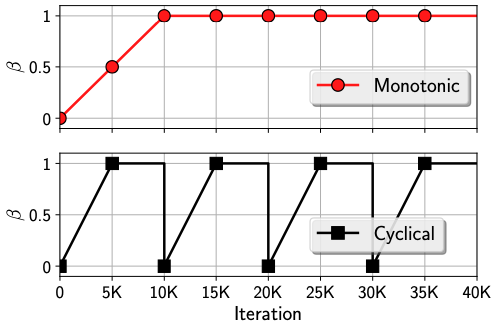
\includegraphics[width=0.5\textwidth]{beta_annealing}
    \caption[Annealing strategy of the KL weight term in variational autoencoders]{Two annealing strategies for the $\beta$ term that weights the KL divergence in the loss function of variational autoencoders. The upper graph shows a monotonic increase of $\beta$, and the lower graph a cyclical annealing strategy. The picture is from \cite{Fu_Li_Liu_Gao_Celikyilmaz_Carin_2019}.}
    \figlbl{beta_annealing}
\end{figure}

In this thesis, $4$ variational autoencoders are used. Each VAE consists of an encoder, two fully-connected layers to calculate $\boldsymbol{\mu}$ and $\boldsymbol{\sigma}$, and a decoder.
The encoder consists of $3$  convolutional layers with $32$, $64$, and $128$ channels. Each convolutional layer has a stride of $2$, halving the input size in each layer.
The decoder has the inverse structure of the encoder, i.e. $3$ transposed convolutional layers with $128$, $64$, and $32$ channels.
The fully connected layer for predicting $\boldsymbol{\mu}$ and $\boldsymbol{\sigma}$ have $32$ neurons.
The network architecture is shown in \figref{horizontal_org_arch1}.

\begin{figure}[h]
    \centering
    \resizebox{0.99\textwidth}{!}
{
\begin{tikzpicture}
\tikzstyle{connection}=[ultra thick,every node/.style={sloped,allow upside down},draw=\edgecolor,opacity=0.7]
\tikzstyle{copyconnection}=[ultra thick,every node/.style={sloped,allow upside down},draw={rgb:blue,4;red,1;green,1;black,3},opacity=0.7]


\node[canvas is zy plane at x=0] (input) at (0,0,0) {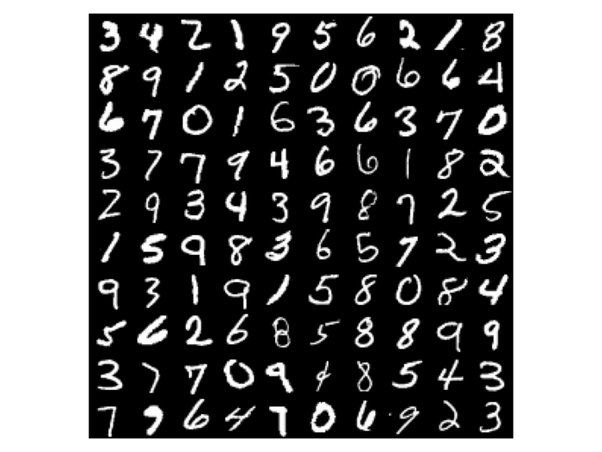
\includegraphics[width=8cm,height=8cm]{imgs/mnist.jpeg}};


\pic[shift={(3,0,0)}] at (input) 
    {Box={
        name=conv1,
        caption=Conv + ReLU,
        xlabel={{1, }},
        zlabel=32,
        fill=\ConvColor,
        height=20,
        width=2,
        depth=20
        }
    };


\draw [connection]  (input) ++(0,0,0)    -- node {\midarrow} (conv1-west);


\pic[shift={(2,0,0)}] at (conv1-east) 
    {Box={
        name=conv2,
        caption=Conv + ReLU,
        xlabel={{32, }},
        zlabel=64,
        fill=\ConvColor,
        height=12,
        width=4,
        depth=12
        }
    };


\draw [connection]  (conv1-east)    -- node {\midarrow} (conv2-west);


\pic[shift={(2,0,0)}] at (conv2-east) 
    {Box={
        name=conv3,
        caption=Conv + ReLU,
        xlabel={{64, }},
        zlabel=128,
        fill=\ConvColor,
        height=6,
        width=6,
        depth=6
        }
    };


\draw [connection]  (conv2-east)    -- node {\midarrow} (conv3-west);


\pic[shift={(2,2,0)}] at (conv3-east) 
    {Box={
        name=fcn1,
        caption=FC + ReLU,
        xlabel={{" ","dummy"}},
        zlabel=32,
        fill=\SoftmaxColor,
        opacity=0.8,
        height=3,
        width=3,
        depth=6
        }
    };


\pic[shift={(2,-2,0)}] at (conv3-east) 
    {Box={
        name=fcn2,
        caption=FC + ReLU,
        xlabel={{" ","dummy"}},
        zlabel=32,
        fill=\SoftmaxColor,
        opacity=0.8,
        height=3,
        width=3,
        depth=6
        }
    };


\draw [connection]  (conv3-east)    -- node {\midarrow} (fcn1-west);


\draw [connection]  (conv3-east)    -- node {\midarrow} (fcn2-west);


\pic[shift={(2,-2,0)}] at (fcn1-east) 
    {Box={
        name=conv4,
        caption=Conv + ReLU,
        xlabel={{128, }},
        zlabel=64,
        fill=\ConvColor,
        height=6,
        width=6,
        depth=6
        }
    };


\draw [connection]  (fcn1-east)    -- node {\midarrow} (conv4-west);


\draw [connection]  (fcn2-east)    -- node {\midarrow} (conv4-west);


\pic[shift={(2,0,0)}] at (conv4-east) 
    {Box={
        name=conv5,
        caption=Conv + ReLU,
        xlabel={{64, }},
        zlabel=32,
        fill=\ConvColor,
        height=12,
        width=4,
        depth=12
        }
    };


\draw [connection]  (conv4-east)    -- node {\midarrow} (conv5-west);


\pic[shift={(2,0,0)}] at (conv5-east) 
    {Box={
        name=conv6,
        caption=Conv + ReLU,
        xlabel={{32, }},
        zlabel=1,
        fill=\ConvColor,
        height=20,
        width=2,
        depth=20
        }
    };


\draw [connection]  (conv5-east)    -- node {\midarrow} (conv6-west);


\node[canvas is zy plane at x=3] (output) at (conv6-east) {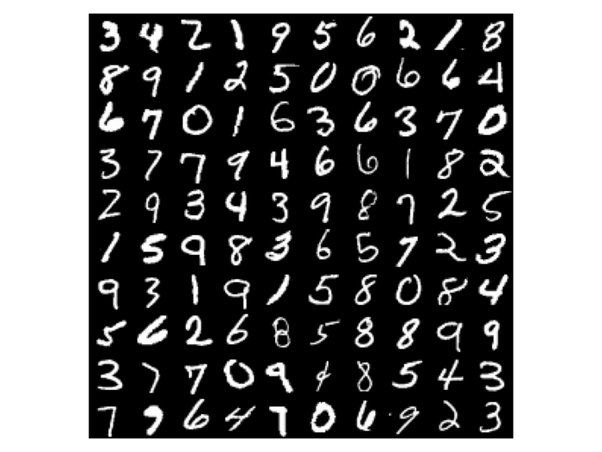
\includegraphics[width=8cm,height=8cm]{imgs/mnist.jpeg}};


\draw [connection]  (conv6-east)     -- node {\midarrow} ($(output) + (0.5,0,0)$);


\end{tikzpicture}
}
    \caption[Architecture of the variational autoencoder used for horizontal self-organisation]{Architecture of the variational autoencoder used for horizontal self-organisation.}
    \figlbl{horizontal_org_arch1}
\end{figure}

Each VAE is trained independently to minimise the loss function as described in \eqref{hso_6}.
Adam \sidecite{Kingma_Ba_2017} is used as an optimisation algorithm with a learning rate of $1\cdot 10^{-3}$, and the mini-batch size is $32$.


\subsection{Predicting bigger Patches}\seclbl{horizontal_self_org_methods_bigger_patches}
Applying monotonic annealing to the KL divergence weight term $\beta$ is the first measure to improve the latent space distribution.
Another measure is to predict bigger patches.
The VAEs have a very limited field of view and cannot distinguish some of the digits on their own (c.f. \secref{horizontal_self_org_methods_communication}).
However, by predicting bigger patches, the VAEs can be encouraged to distinguish similar-looking patches better.
For example, the patches for the digits $4$, $5$, and $6$ look very similar for the first VAE that receives the patch extracted from the top left corner of the samples (c.f. \figref{average_sample}).
Since the target prediction of these two digits is similar, they are located closely together in the latent space.
When a VAE predicts bigger patches or the entire image, the target predictions of the digits $4$, $5$, and $6$ become different. Thus, while similar latent representations are sufficient to predict only a patch of these digits, predicting larger patches or the whole picture requires more separated latent representations.
Thus, predicting bigger patches helps push apart latent representations of objects with a high patch-wise similarity but a low image-wise similarity.


In this thesis, an additional layer is used in the decoder to predict larger patches. In fact, the last layer with $32$ channels and a stride of $2$ is used twice so that the decoder has $4$ transposed convolutional layers with $128$, $64$, $32$, and $32$ channels. Thus, the output size of the decoder is doubled. This architecture is shown in Figure \figref{horizontal_org_arch2}.


\begin{figure}[h]
    \centering
    \resizebox{0.99\textwidth}{!}
{
\begin{tikzpicture}
\tikzstyle{connection}=[ultra thick,every node/.style={sloped,allow upside down},draw=\edgecolor,opacity=0.7]
\tikzstyle{copyconnection}=[ultra thick,every node/.style={sloped,allow upside down},draw={rgb:blue,4;red,1;green,1;black,3},opacity=0.7]


\node[canvas is zy plane at x=0] (input) at (0,0,0) {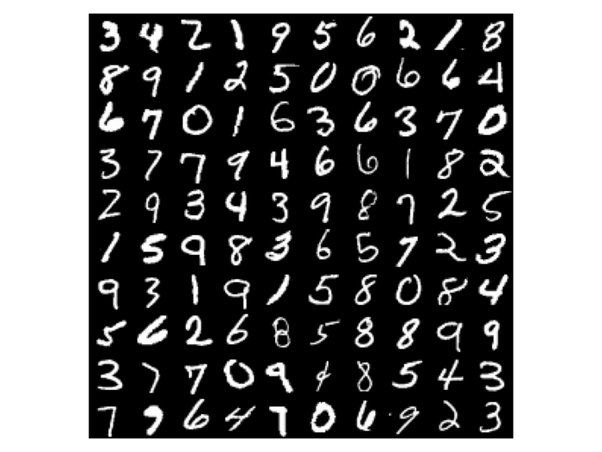
\includegraphics[width=8cm,height=8cm]{imgs/mnist.jpeg}};


\pic[shift={(3,0,0)}] at (input) 
    {Box={
        name=conv1,
        caption=Conv + ReLU,
        xlabel={{1, }},
        zlabel=32,
        fill=\ConvColor,
        height=20,
        width=2,
        depth=20
        }
    };


\draw [connection]  (input) ++(0,0,0)    -- node {\midarrow} (conv1-west);


\pic[shift={(2,0,0)}] at (conv1-east) 
    {Box={
        name=conv2,
        caption=Conv + ReLU,
        xlabel={{32, }},
        zlabel=64,
        fill=\ConvColor,
        height=12,
        width=4,
        depth=12
        }
    };


\draw [connection]  (conv1-east)    -- node {\midarrow} (conv2-west);


\pic[shift={(2,0,0)}] at (conv2-east) 
    {Box={
        name=conv3,
        caption=Conv + ReLU,
        xlabel={{64, }},
        zlabel=128,
        fill=\ConvColor,
        height=6,
        width=6,
        depth=6
        }
    };


\draw [connection]  (conv2-east)    -- node {\midarrow} (conv3-west);


\pic[shift={(2,2,0)}] at (conv3-east) 
    {Box={
        name=fcn1,
        caption=FC + ReLU,
        xlabel={{" ","dummy"}},
        zlabel=32,
        fill=\SoftmaxColor,
        opacity=0.8,
        height=3,
        width=3,
        depth=6
        }
    };


\pic[shift={(2,-2,0)}] at (conv3-east) 
    {Box={
        name=fcn2,
        caption=FC + ReLU,
        xlabel={{" ","dummy"}},
        zlabel=32,
        fill=\SoftmaxColor,
        opacity=0.8,
        height=3,
        width=3,
        depth=6
        }
    };


\draw [connection]  (conv3-east)    -- node {\midarrow} (fcn1-west);


\draw [connection]  (conv3-east)    -- node {\midarrow} (fcn2-west);


\pic[shift={(2,-2,0)}] at (fcn1-east) 
    {Box={
        name=conv4,
        caption=Conv + ReLU,
        xlabel={{128, }},
        zlabel=64,
        fill=\ConvColor,
        height=6,
        width=6,
        depth=6
        }
    };


\draw [connection]  (fcn1-east)    -- node {\midarrow} (conv4-west);


\draw [connection]  (fcn2-east)    -- node {\midarrow} (conv4-west);


\pic[shift={(2,0,0)}] at (conv4-east) 
    {Box={
        name=conv5,
        caption=Conv + ReLU,
        xlabel={{64, }},
        zlabel=32,
        fill=\ConvColor,
        height=12,
        width=4,
        depth=12
        }
    };


\draw [connection]  (conv4-east)    -- node {\midarrow} (conv5-west);


\pic[shift={(2,0,0)}] at (conv5-east) 
    {Box={
        name=conv6,
        caption=Conv + ReLU,
        xlabel={{32, }},
        zlabel=32,
        fill=\ConvColor,
        height=20,
        width=2,
        depth=20
        }
    };


\draw [connection]  (conv5-east)    -- node {\midarrow} (conv6-west);


\pic[shift={(2,0,0)}] at (conv6-east) 
    {Box={
        name=conv7,
        caption=Conv + ReLU,
        xlabel={{32, }},
        zlabel=1,
        fill=\ConvColor,
        height=20,
        width=2,
        depth=20
        }
    };


\draw [connection]  (conv6-east)    -- node {\midarrow} (conv7-west);


\node[canvas is zy plane at x=3] (output) at (conv7-east) {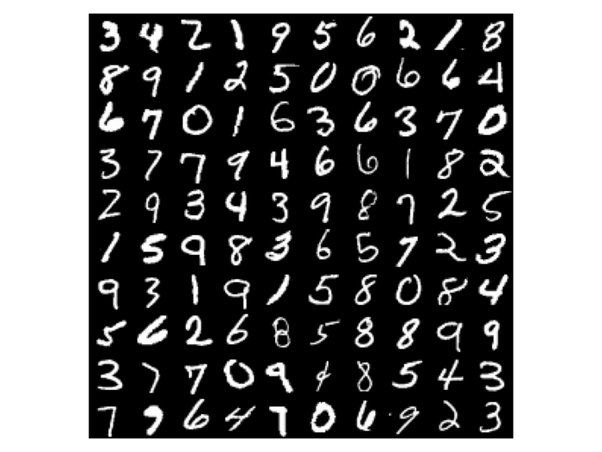
\includegraphics[width=8cm,height=8cm]{imgs/mnist.jpeg}};


\draw [connection]  (conv6-east)     -- node {\midarrow} ($(output) + (0.5,0,0)$);


\end{tikzpicture}
}
    \caption[Architecture of the VAE used for horizontal self-organisation with bigger field-of-view up-sampling]{Architecture of the variational autoencoder used for horizontal self-organisation with bigger field-of-view up-sampling.}
    \figlbl{horizontal_org_arch2}
\end{figure}

When using $4$ VAEs, the input is divided into $4$ patches. If the decoder makes the output twice as large as the input by up-sampling,  the entire image is predicted by each of the VAEs. This process is visualised in \figref{bigger_patches}.

\begin{figure}[h]
    \centering
    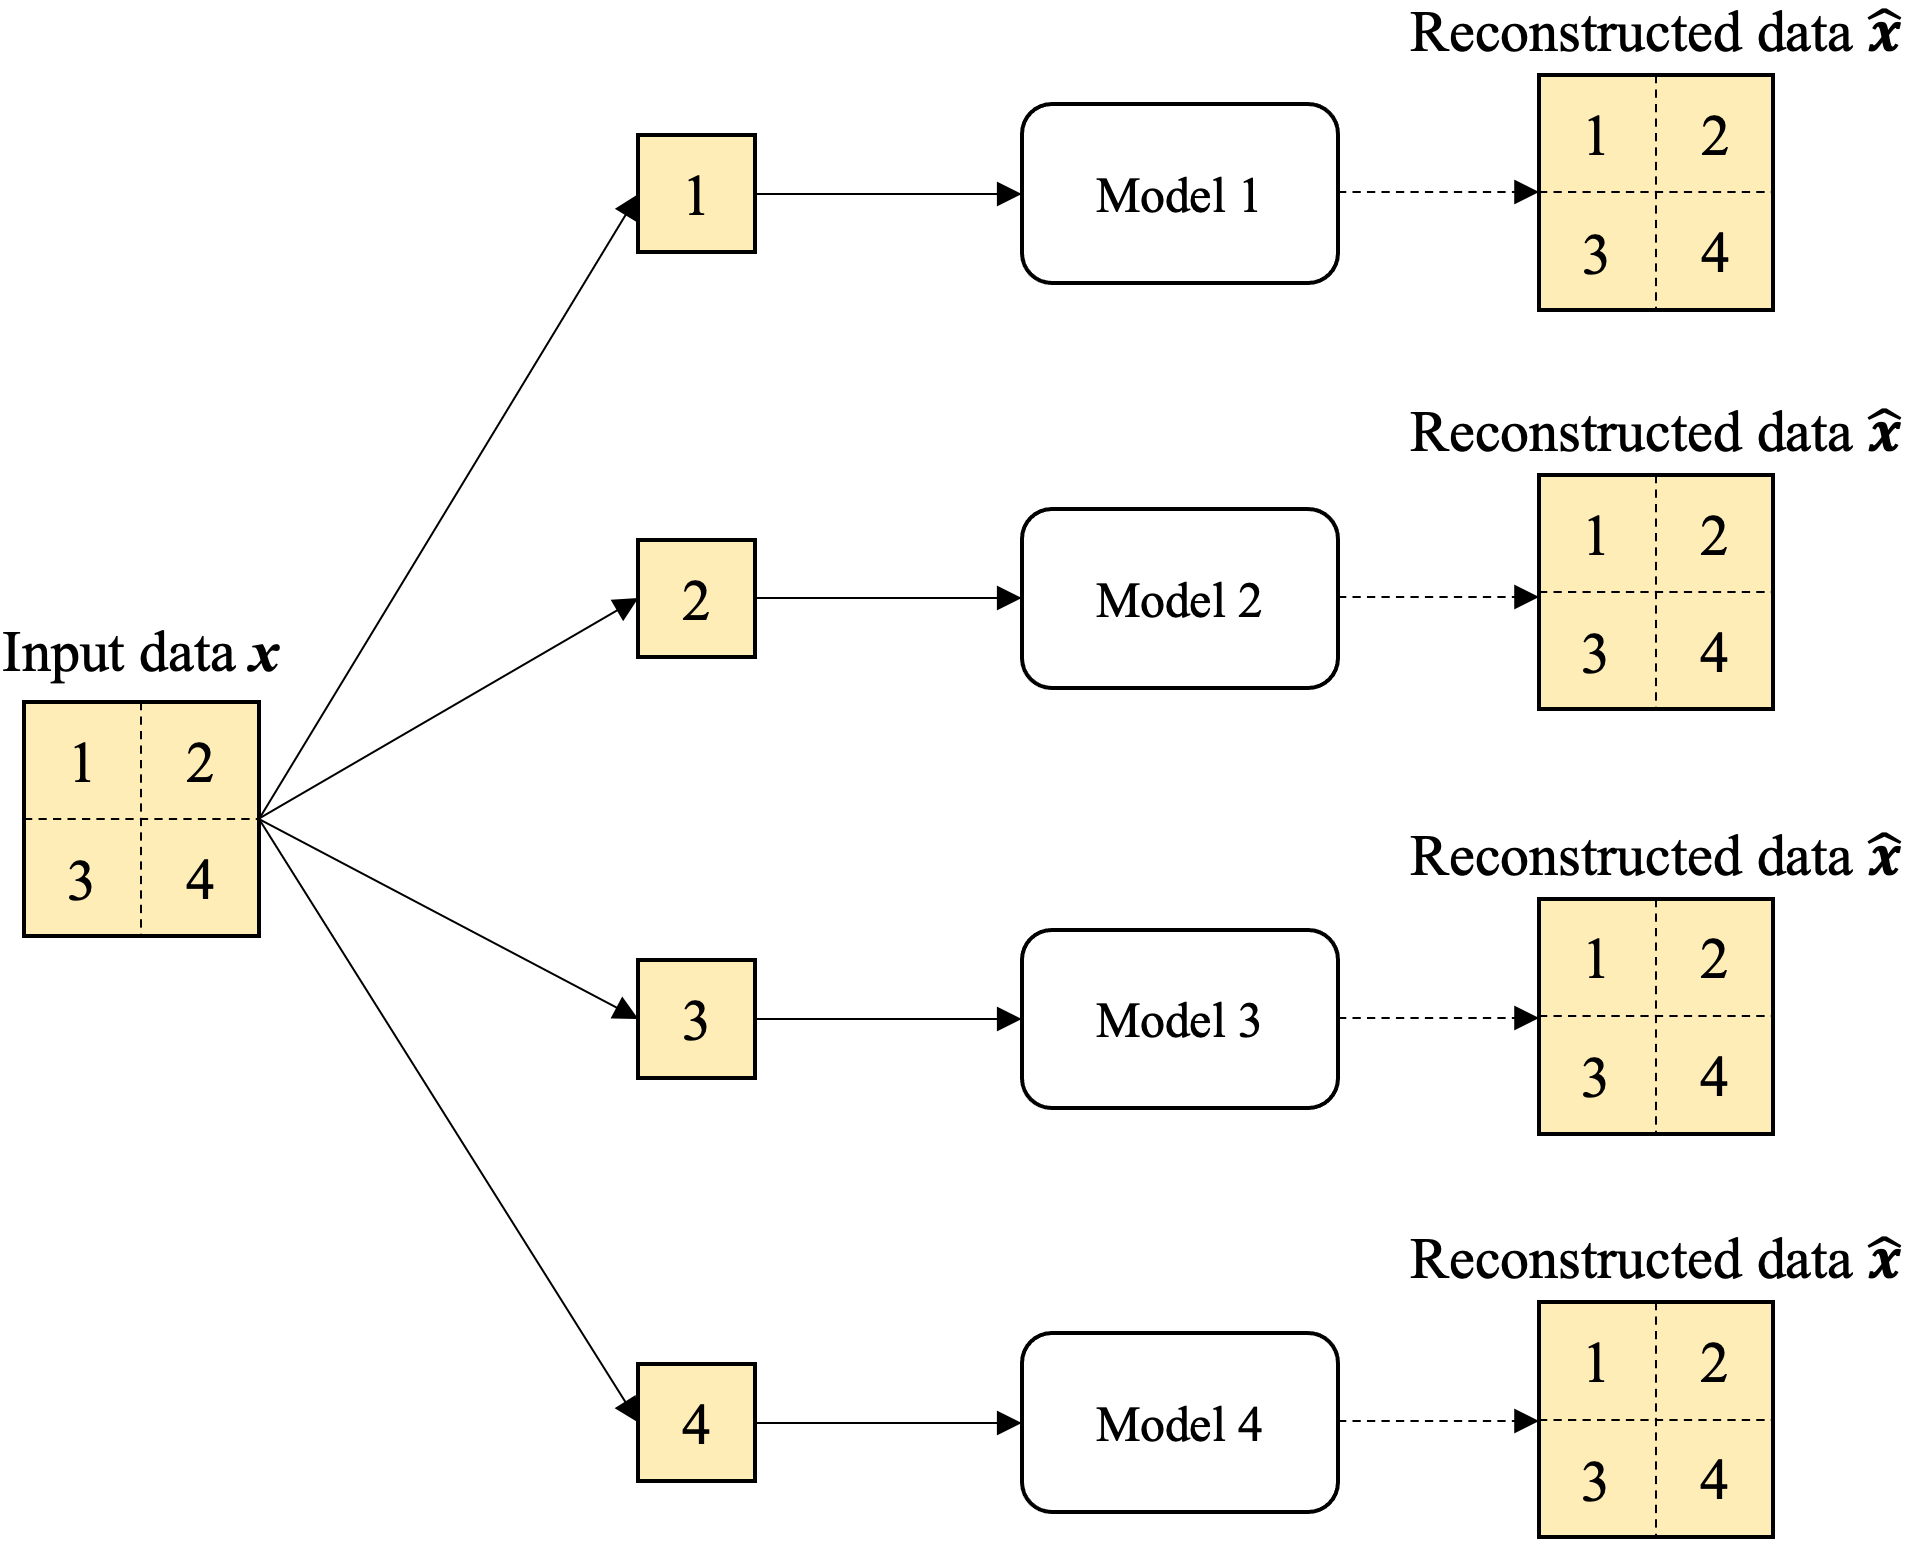
\includegraphics[width=0.99\textwidth]{bigger_patches}
    \caption[Reconstruction of bigger output than input patches]{Four models receive a quarter of the image as input patch to predict the entire image.}
    \figlbl{bigger_patches}
\end{figure}



\subsection{Communication}\seclbl{horizontal_self_org_methods_communication}
The VAEs receive patches of the input image and thus have a limited field of view on the image.
Figure \figref{average_sample} visualises the patches that are fed into the VAEs when the MNIST data set \cite{Lecun_Bottou_Bengio_Haffner_1998} is used.
The first row shows the average of all images of the same class. Thus, these images are very representative for the data set.
However, none of the models receives the entire image as input. Instead, the patches shown in the 2nd to the 5th row are fed into the VAEs.
The patches, which only depict a quarter of the image, look rather similar for some classes. For example, the top-left patches of the classes $0$ and $9$, as well as the classes $4$, $5$, and $6$, look very similar.
Thus, these classes are not separable by \emph{one} single VAE on its own.
Therefore, communication with neighbouring models is necessary to agree on an image representation.

\begin{figure}[h]
    \centering
    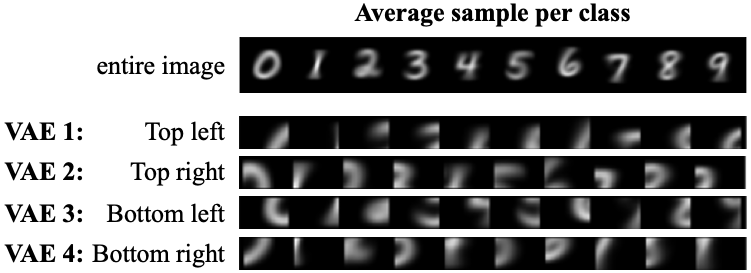
\includegraphics[width=0.99\textwidth]{average_sample}
    caption[Average sample of the MNIST data set per class]{The average of all samples in the MNIST data set for each class. The first row shows the average of all samples, and the 2nd to 5th row is the average per patch fed into the models.}
    \figlbl{average_sample}
\end{figure}


This concept links well to the biological model: A single VAE can be seen as a neuron or a group of neurons. Initially, the VAEs have many suggestions to which classes the received patch could belong. However, through communication with neighbouring VAEs, suggestions are constantly ruled out because neighbouring VAEs do not support them. Thus, out of many suggestions, only the most valid ones are retained, resulting in an image representation. The biological model behaves similarly: At first, many neurons are active because they are excited by the captured image. However, this strong activation quickly becomes sparse as only the neurons supporting each other remain active. This process leads to the emergence of higher-level features (i.e. net fragments) that are representative of the captured input \sidecite{Malsburg_1987}.

One of the biggest strengths of autoencoders is that they do not rely on labels but can be trained in an unsupervised manner. To keep this strength, also communication should not rely on labels. Therefore, different types of communication are proposed that work without labels: communication based on latent representations, communication based on reconstructed images, and communication via a dedicated communication channel.

All these types of communication take place over two or more time steps. First, image patches are reconstructed by all VAEs. As a result, each VAE generates information in latent space. Then, this information can be communicated to the neighbouring VAEs. Thus, in a second time-step, the VAEs have more information available: their prediction is based on the reconstructed image patch and information from neighbouring VAEs. This additional information allows them to improve their prediction. The process can be repeated over a fixed number of time steps or until the network reaches an attractor state (i.e. the latent representations no longer change). In the following, different types of communication are proposed.


\subsubsection{Model Heads}
Each VAE learns the mapping from a patch to a latent space with Gaussian distribution, i.e. obtains a $\boldsymbol{mu}$ and $\boldsymbol{sigma}$ for each sample that is used to predict a reconstructed version of the input.
The arrangement of the representations within the latent space is not predetermined by an external system but is fself-organised. A consequence of independent systems is that $\boldsymbol{mu}$ and $\boldsymbol{sigma}$ have different meanings in the latent spaces of different VAEs. Thus, one VAE cannot interpret the Gaussian parameters of another VAE.

In this thesis, it is proposed to learn a linear transformation to map the Gaussian parameters of one VAE to the Gaussian parameters of another VAE. The mapping from $\boldsymbol{mu}_1$ to $\boldsymbol{mu}_2$, respectively from $\boldsymbol{sigma}_1$ to $\boldsymbol{sigma}_2$ is done by the simple transformation

\begin{equation}\eqlbl{hso_7}
	\boldsymbol{\hat{\mu}}_2 = \boldsymbol{w}_{m12} \cdot \boldsymbol{\mu}_1
\end{equation}

resp.

\begin{equation}\eqlbl{hso_8}
	\boldsymbol{\hat{\sigma}}_2 = \boldsymbol{w}_{s12} \cdot \boldsymbol{\sigma}_1
\end{equation}

The weights $\boldsymbol{w}_{mij}$ and $\boldsymbol{w}_{sij}$ between VAE $i$ and VAE $j$ are learned by minimising the mean square error with gradient descent between the predicted and true Gaussian parameters, i.e. between $\boldsymbol{\mu}_j$ and $\boldsymbol{\hat{\mu}}_j$, resp. $\boldsymbol{\sigma}_j$ and $\boldsymbol{\hat{\sigma}}_j$. This process is illustrated for VAE 1 in \figref{hso_head}: First, the Gaussian parameters of each model must be predicted for the same sample. Afterwards, the Gaussian parameters of one model can be used to predict the Gaussian parameters of the other models with a linear transformation.

\begin{figure}[h]
    \centering
    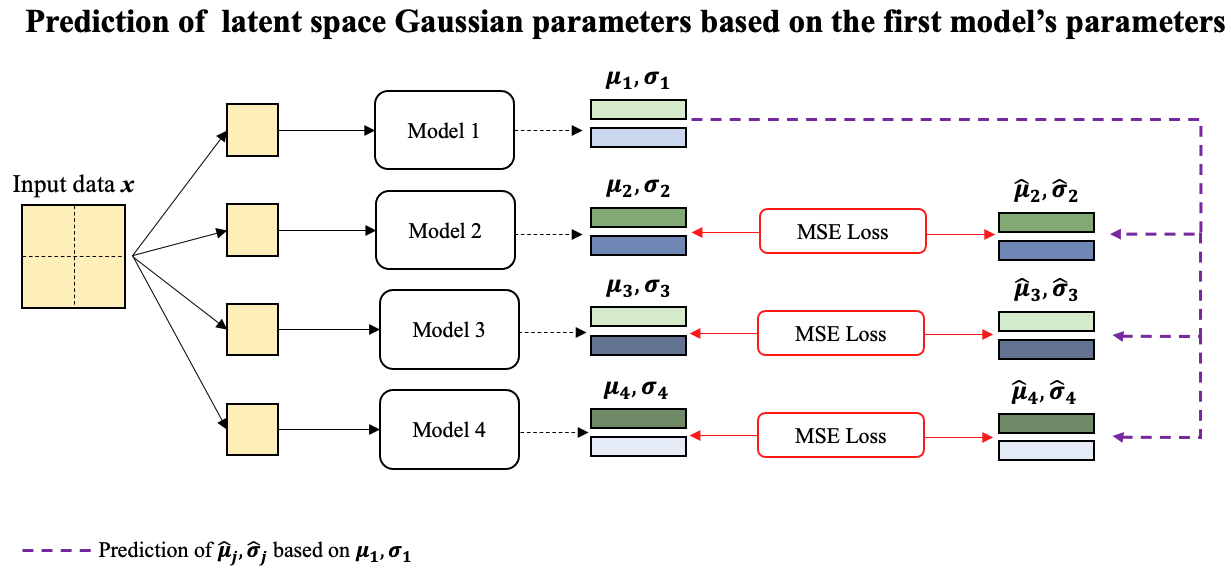
\includegraphics[width=0.99\textwidth]{hso_head}
    \caption[Prediction of Gaussian parameters of other VAEs]{Visualisation of how the first VAE can predict the Gaussian parameters of the other VAEs.}
    \figlbl{hso_head}
\end{figure}

If each VAE predicts the Gaussian parameters of the other VAEs, then these predictions can be communicated, and each VAE receives further suggestions from neighbouring VAEs. Thus, each VAE has its own calculated Gaussian parameters and suggestions from neighbours about what its Gaussian parameters might be. This allows a VAE to correct its prediction. Each VAE receives additional information because the suggestions made by neighbouring VAEs are based on a different patch. For example, the VAE that sees only one patch from the top left of the image cannot distinguish the digits $5$ and $6$. On the other hand, the VAE that sees the patch at the bottom left can distinguish these digits. Thus, the VAE at the bottom left can help the VAE at the top left to choose a better latent representation.

TODO: At the moment, various experiments are still ongoing to find out how this can be implemented (therefore, not yet explained in more detail).




















\subsubsection{Reconstructed Images}
As described in \secref{horizontal_self_org_methods_bigger_patches}, the prediction of larger patches helps to better arrange the latent space. The prediction of larger patches can also be used for communication with neighbouring VAEs. Instead of extracting representations from the latent space and transmitting them to neighbouring VAEs as described in the last section, the reconstructed image can also be exchanged. This is done by predicting a part of the image in a first time-step and by adding this prediction to an additional input channel of another VAE in the next time-step. Various data can be forwarded to other VAEs:% and is explained below. Let $\boldymbol{x}$ be the input image and $\boldymbol{\hat{x}}$ the reconstructed image. For $n$ VAEs, the input sample $\boldymbol{x}$ is split into $n$ non-overlapping patches $\boldymbol{x}^{(1)}, ..., \boldymbol{x}^{(n)}$. The reconstructed patches are denoted as $\boldymbol{\hat{x}}^{(1)}, ..., \boldymbol{\hat{x}}^{(n)}$. If a VAE reconstructs the same patch as it received as input, $\boldymbol{x}^{(i)} \approx \boldymbol{\hat{x}}^{(i)}$ is valid. However, when a bigger patch is predicted than the one that was fed into the model, then this term is not valid anymore, i.e. $\boldymbol{x}^{(i)} \not\approx \boldymbol{\hat{x}}^{(i)}$. However, if only a part of the prediction $\boldymbol{\hat{x}}^{(i)}$ is considered (i.e. the prediction is cropped), then $\boldymbol{x}^{(i)}$ is contained in this cropped version of the prediction $\boldymbol{\hat{x}}^{(i)}_C$.


\begin{figure}
    \centering
    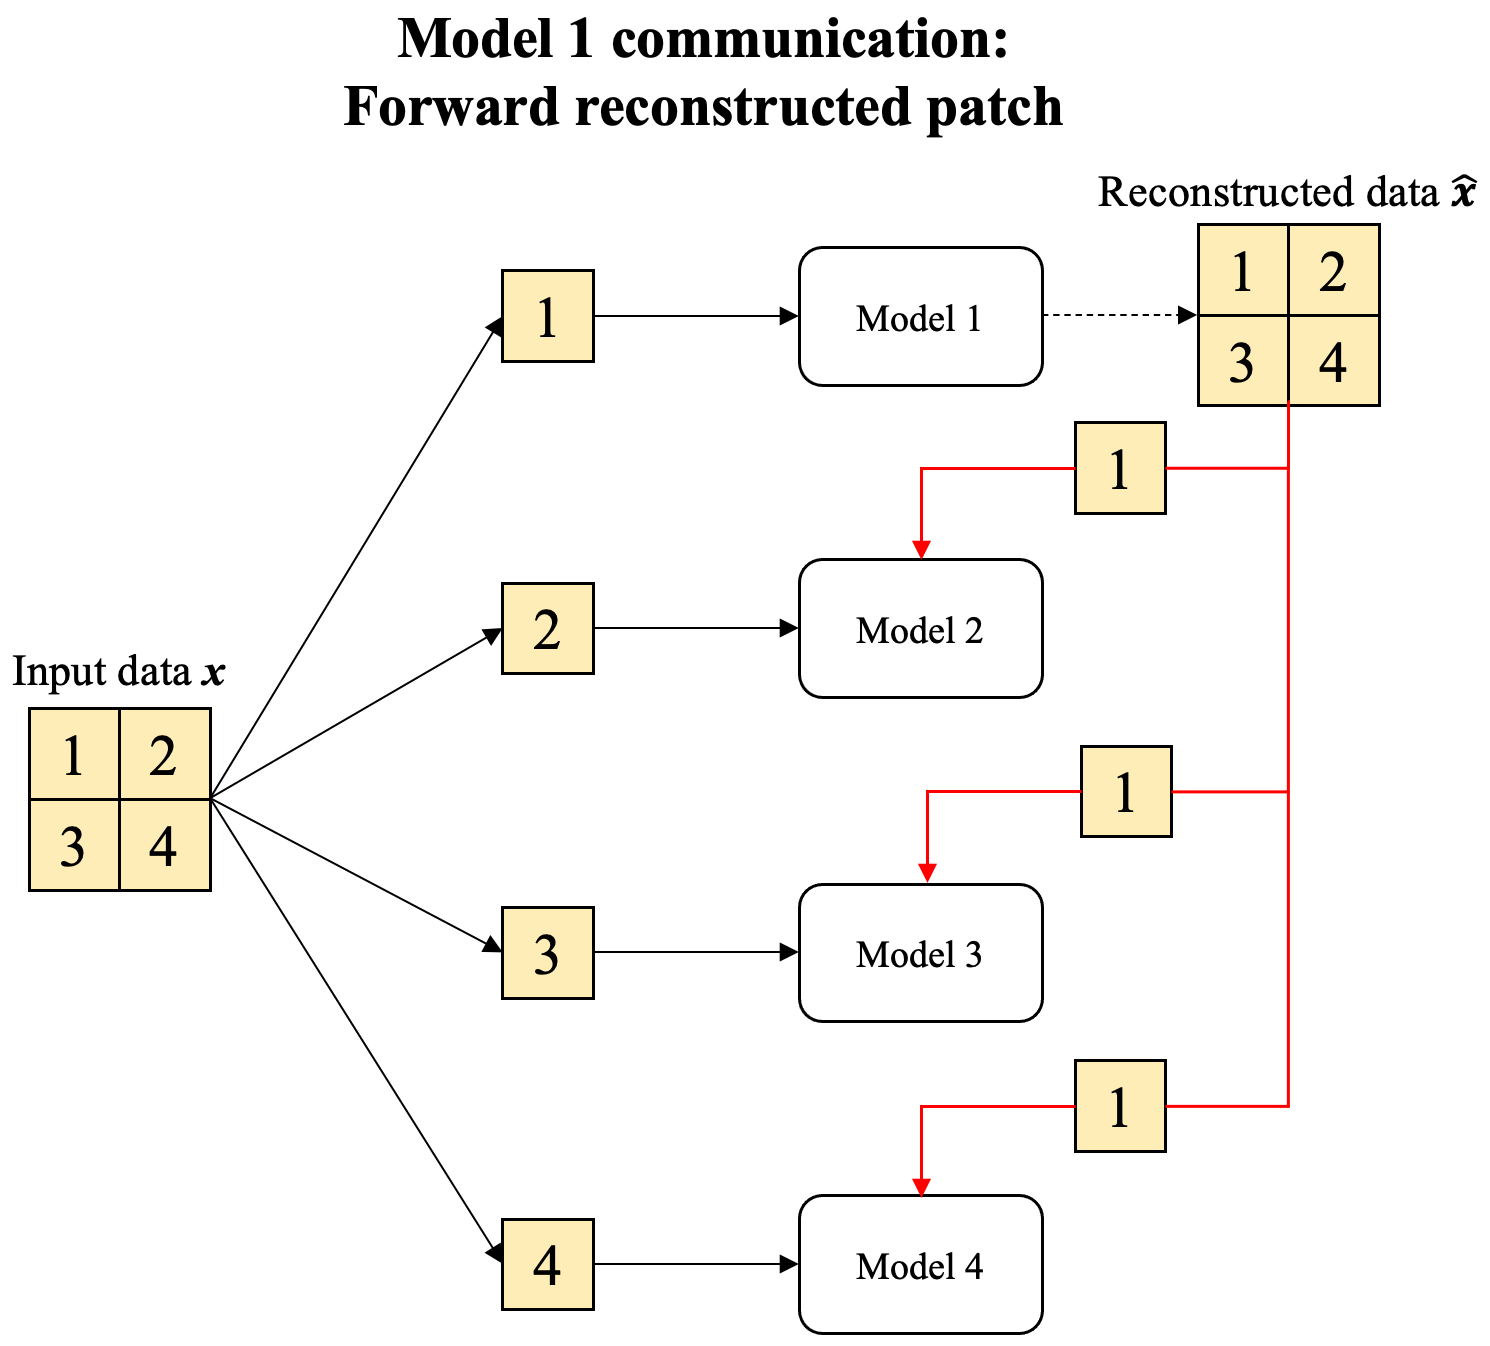
\includegraphics[width=0.80\textwidth]{recon_patch_forw}
    \caption[Communication between VAEs by forwarding reconstructed patch]{Communication between VAEs by forwarding reconstructed patch, example on the basis of the first VAE: The first VAE predicts the image and forwards the reconstructed patch (the same patch that was fed into the model) to the other VAEs.}
    \figlbl{recon_patch_forw}
\end{figure}

\begin{figure}
    \centering
    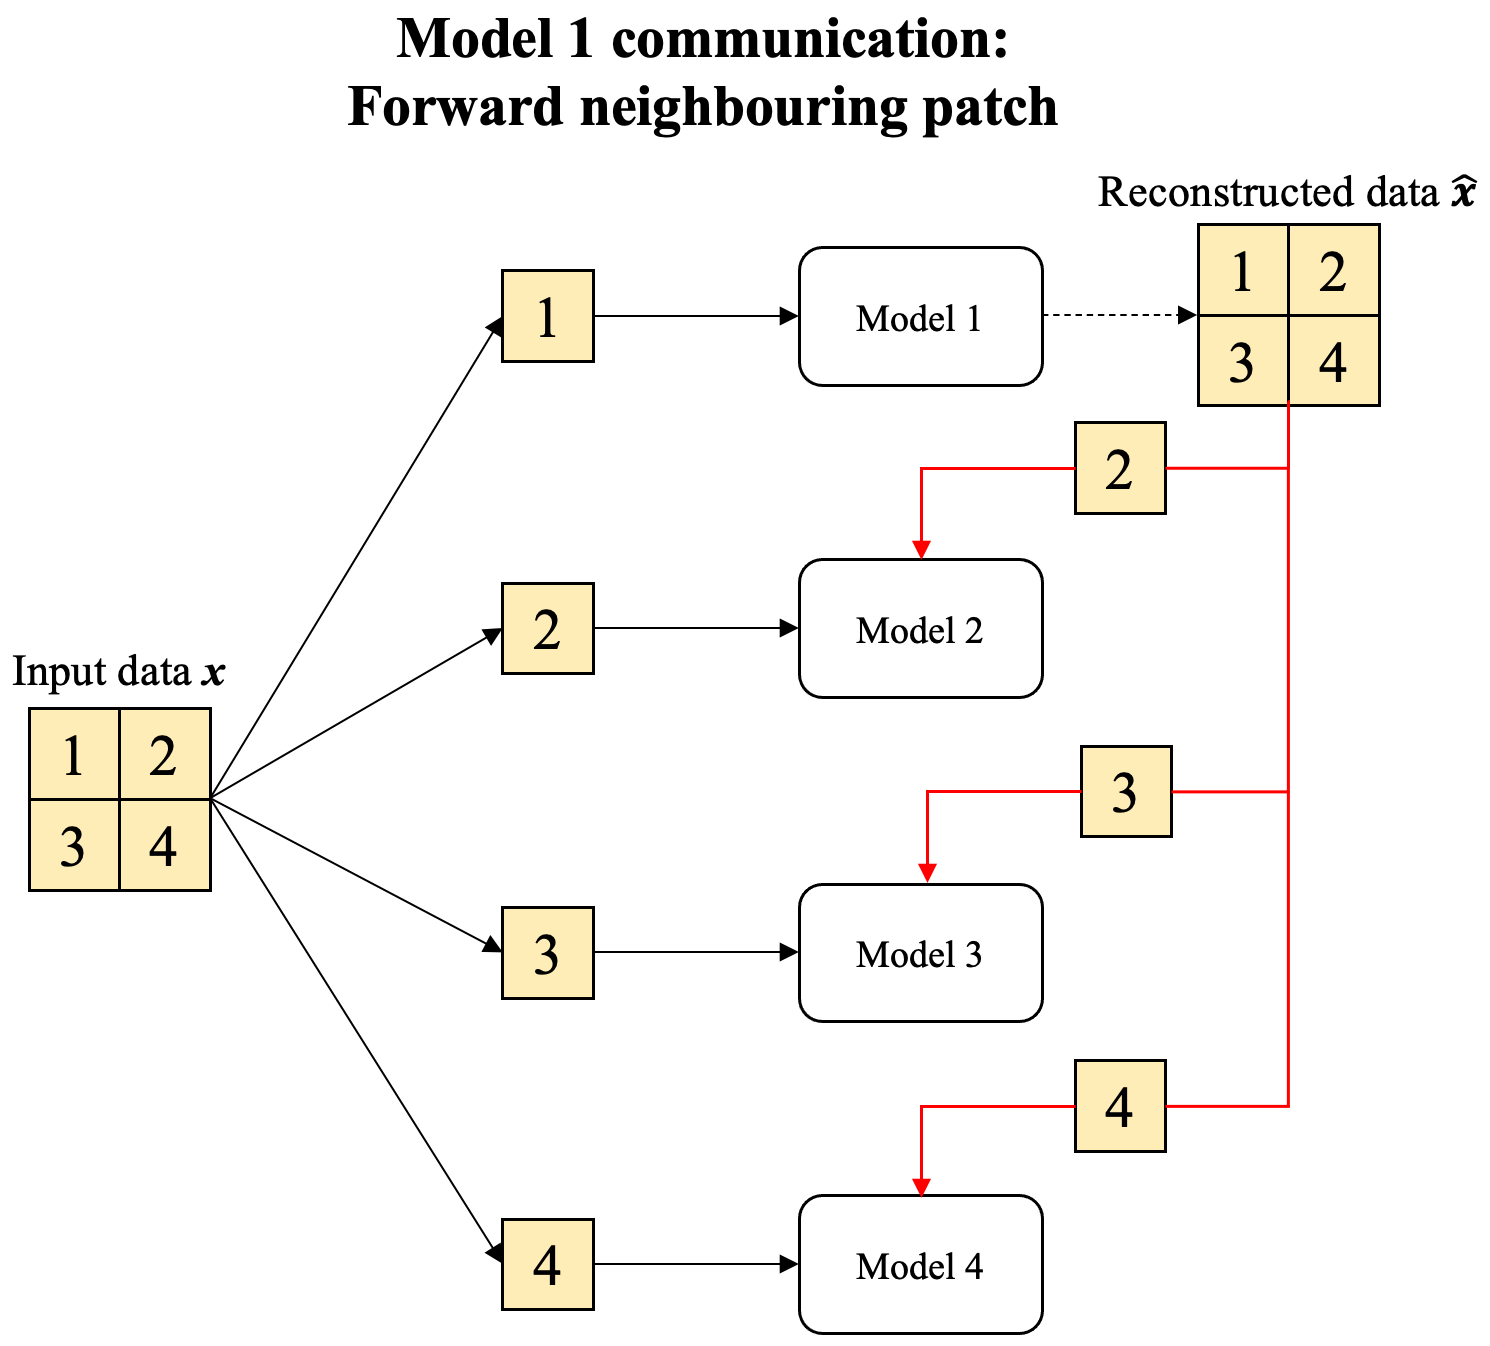
\includegraphics[width=0.80\textwidth]{neighbouring_patch_forw}
    \caption[Communication between VAEs by forwarding prediction of neighbouring patches]{Communication between VAEs by forwarding prediction of neighbouring patches, example on the basis of the first VAE: The first VAE predicts the image and forwards a prediction of how the neighbourhood could look like to the other VAEs. Thus, each other VAE receives a patch and a prediction of the first VAE how this patch could look like as input.}
    \figlbl{neighbouring_patch_forw}
\end{figure}

\begin{figure}
    \centering
    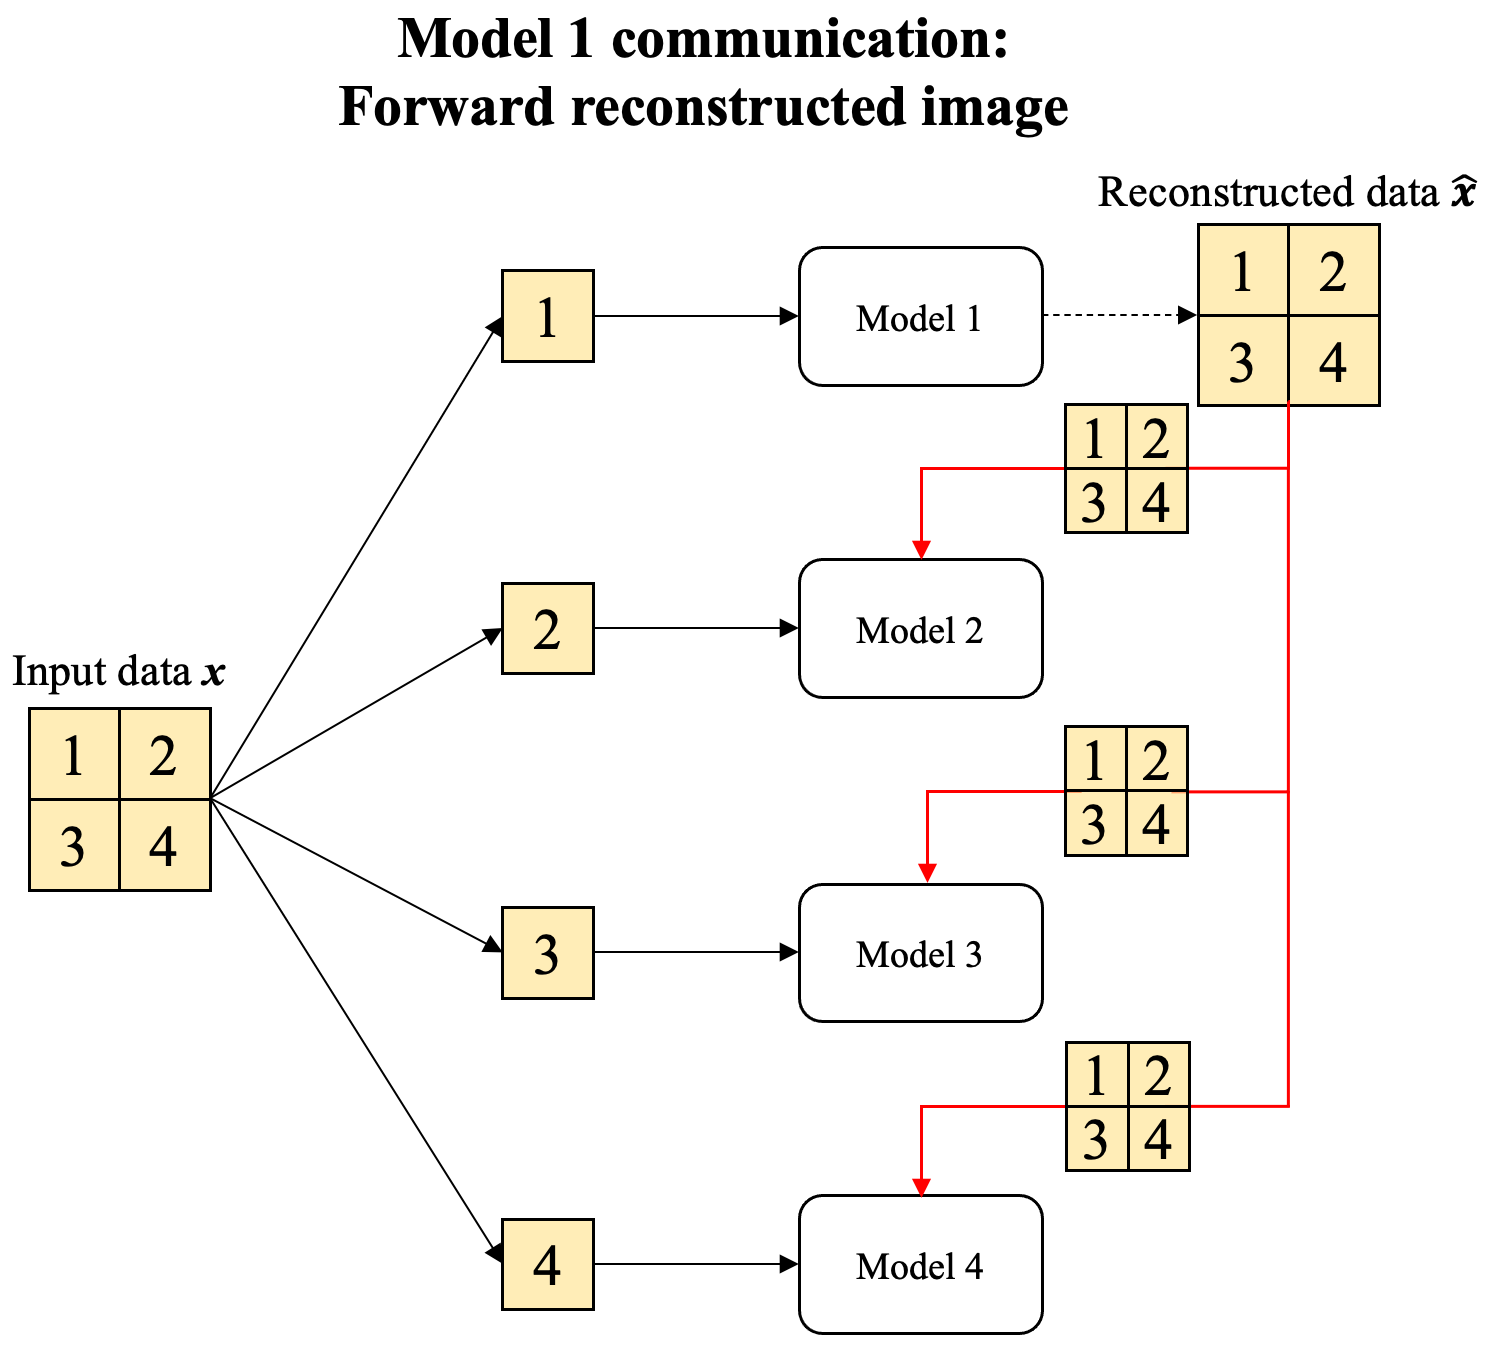
\includegraphics[width=0.80\textwidth]{recon_img_forw}
    \caption[Communication between VAEs by forwarding prediction of the entire image]{Communication between VAEs by forwarding prediction of the entire image, example on the basis of the first VAE: The first VAE predicts the image and forwards the prediction of the image to the other VAEs.}
    \figlbl{recon_img_forw}
\end{figure}



\begin{description}
	\item [Reconstructed Patch] Each VAE reconstructs its input patch and optionally a part of the neighbourhood. It tells the other VAEs what the reconstructed version of its input patch looks like. Information about the optionally reconstructed neighbourhood is not communicated to other VAEs. Thus, a reconstructed version of the input is sent to other VAEs and added as a new channel to their input. This process is exemplified for the first VAE in \figref{recon_patch_forw}. The problem with this approach is that in the first time-step all VAEs reconstruct their patch and the reconstructed version is communicated to the neighbouring VAEs. As a result, in the second time-step, each VAE receives information about the entire image and thus has access to global instead of only local image information\sidenote{even with a very large number of VAEs and communication restricted to the local neighbourhood, information about the entire image propagates to all VAEs over time, provided enough time-steps are executed}.  
	\item [Neighbouring Patch] Instead of communicating the reconstructed input patch to the neighbours, a prediction can be made of what the input patch of the neighbour looks like and this prediction can be communicated. This has the advantage that each UAE receives different versions of the same patch as input and thus has no global image information. This process for the first VAE is visualised in \figref{neighbouring_patch_forw}. Intuitively, this can solve the following problem: If a VAE cannot decide which digit to predict, neighbouring VAEs can help it by predicting its input patch in a form that is more similar to one of the digits and thus support the VAE by making its decision. 
	\item[Entire image] The simplest version is when each VAE predicts the entire image and communicates this to all other VAEs. In the first time-step, only local information is available, in the second time-step, various predictions of how the image could look are additionally provided. Each VAE can then correct its own prediction based on these predictions of the other VAEs. This process is represented in \figref{recon_img_forw}. Identical to ``reconstructed patches'', global image information is made available to each VAE. This problem can be alleviated if for each VAE $i$ that receives the input patch $\boldsymbol{x}^{(i)}$, the part from its prediction of the whole image corresponding to $\boldsymbol{x}^{(i)}$ is masked. Otherwise, an input patch of a VAE is fed through the encoder and decoder and then communicated to the other VAEs. Then implicitly reconstructed data and not just neighbourhood predictions gets to each VAE as input. 
\end{description}



\subsubsection{Communication Channel}
Another way to communicate is through a dedicated communication channel. For this purpose, each VAE has not only $1$ input and $1$ output channel but $4$ input and output channels. The input patch is fed into the first channel and a reconstructed version of it is predicted in the first output channel. This corresponds to a classic VAE and the loss function remains identical.
The remaining three channels are for communication: Each VAE generates a separate communication output for its $3$ neighbouring VAEs on the remaining $3$ channels. Each of these channels is then stacked to the input of the corresponding VAE. For example, the first VAE receives a given patch on the input channel $1$ and communication data from the 2nd, 3rd, and 4th VAE on the input channels $2$-$4$. Based on this information, it outputs a reconstruction of the patch on the output channel $1$ and communication data to the 2nd, 3rd, and 4th VAE on the output channels $2$-$4$. Thus, there is a dedicated two-way communication channel between each neighbouring VAE. This is shown in \figref{vae_comm_channel}.


\begin{figure}[h]
    \centering
    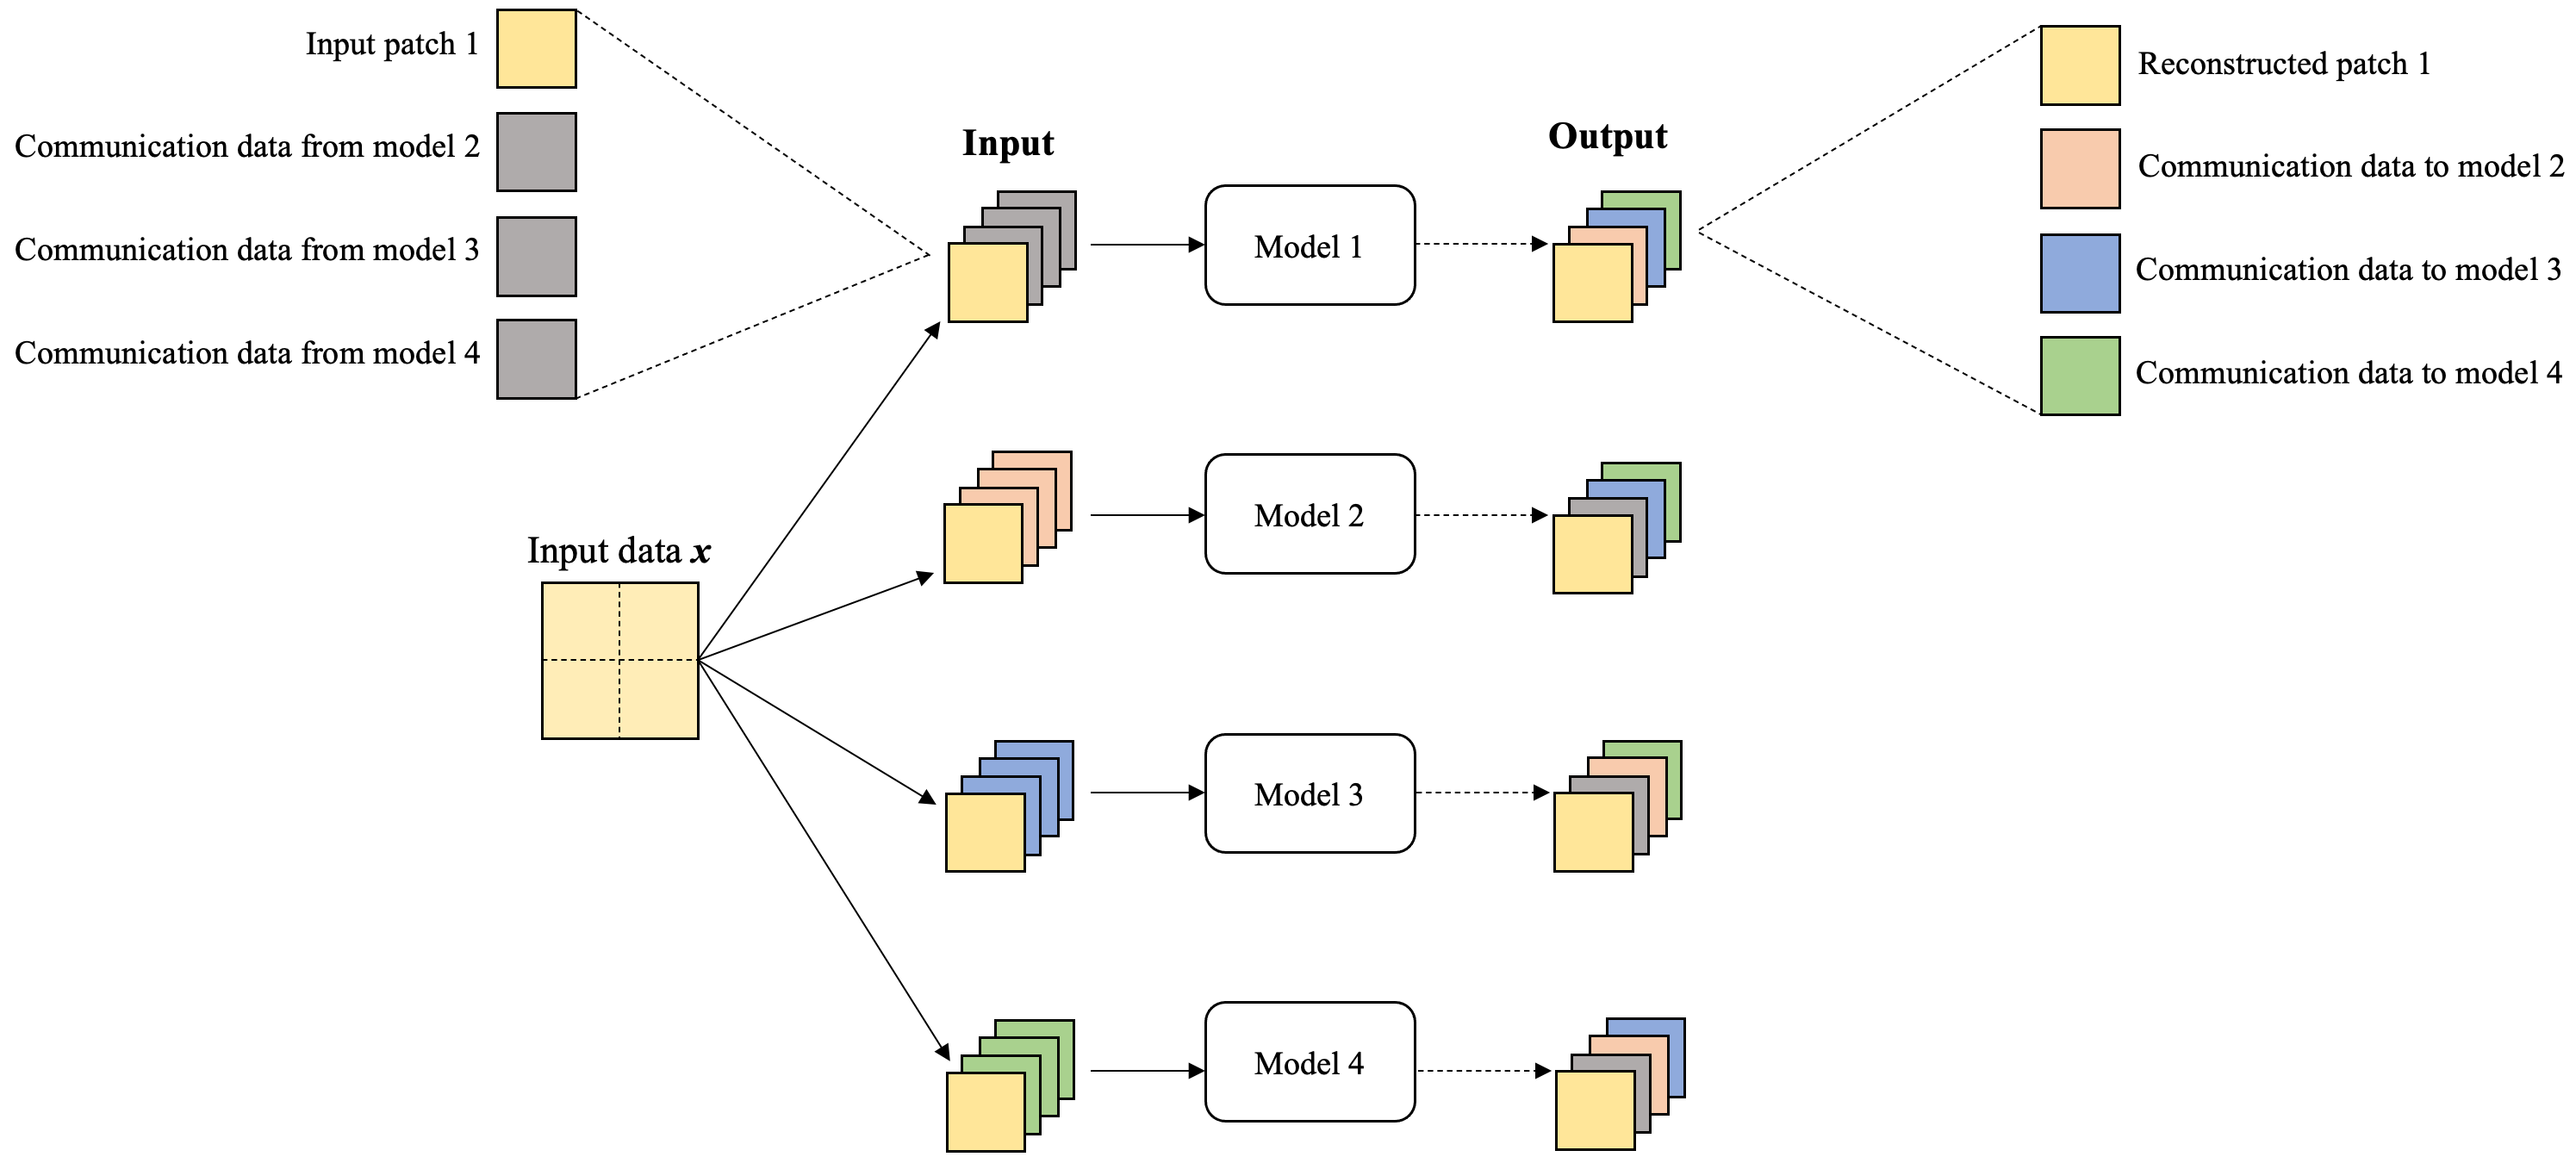
\includegraphics[width=0.89\textwidth]{vae_comm_channel}
    \caption[Communication between VAEs with a dedicated communication channel]{Each VAE has one and output channel to receive and reconstruct a given image patch. The other input and output channels are used for communication: Each VAE has for each other VAE a separate output channel to send messages and an additional input channel to receive messages.}
    \figlbl{vae_comm_channel}
\end{figure}

The loss function remains the same for the first output channel since the goal is still the same, i.e. to reconstruct the output as good as possible. The only difference is that model can now access $4$ input channels to reconstruct the input instead of one channel. However, the communication channels must be trained in order for them to be helpful for input reconstruction. Therefore, an additional loss term is applied on the $3$ output communication channels. Thereby, the idea is to optimize the output of these communication channels in a way so that the other VAEs can better reconstruct their patch.

Let $V = {V_1, ..., V_n}$ be the set of $n$ VAEs. Each VAE has $n$ output channels, one channel for the reconstructed image and $n-1$ channels for communication. Furthermore, each VAE $V_i$ has a loss $L_{\text{VAE}_i}$ based on the reconstruction goodness and the shape of the latent space (c.f. \eqref{hso_6}). The $3$ communication channels of a VAE $i$ can influence the loss $L_{VAE_j}$ of VAE $j$ (i.e. help to improve the loss by providing better information). How helpful the communication channels are can therefore be determined by the average of the loss of the other VAEs.

\begin{equation}\eqlbl{hso_9}
	L_{c_i} = \frac{1}{n-1} \sum_{n}^{j=1} L_{\text{VAE}_j} \text{, if } i \neq j
\end{equation}

Thus, the loss of a VAE with communication channel is

\begin{equation}\eqlbl{hso_10}
		L_{{\text{VAE}_C}_i} = L_{\text{VAE}_i} + \beta \cdot L_{\text{KLD}_i} + \beta_2 \cdot L_{c_i}
\end{equation}

where $\beta_2$ is a weight factor for the communication channel. Thus, each model optimizes its own reconstruction error, the shape of the latent space, and tries to improve the latent space and reconstruction error of other VAEs.


TODO: This has not been implemented yet (therefore, not explained in more detail).


\subsection{Class Prediction}
The VAEs are examined whether they are suitable for predicting the class label. To do this, all VAEs are first trained until they can reliably reconstruct images and the latent space is well formed.
After training, the average value of $\boldsymbol{\mu}$ is determined for each class $c \in C$ from the training set and each VAE $v$. This average value is called $\boldsymbol{\mu}_{\text{avg}_c}$ and is defined for $n$ samples as

\begin{equation}\eqlbl{hso_12}
		\boldsymbol{\mu}_{\text{avg}_vc} = \frac{1}{n} \sum_{i=1}^{n} \boldsymbol{\mu}_i
\end{equation}

This average value can be considered as the ``cluster centre'' of a class in latent space. In addition, $\boldsymbol{\mu}_{\text{avg}_vc}$ is a world model of a class. To make a prediction, a given sample is matched against these world models per class. As with vertical self-organisation, the cosine similarity between a sample and the class prototypes is used to determine their similarity. To predict a sample, first its $\boldsymbol{\mu}_vs$ is determined. Then, this sample is compared with all classes by computing the cosine similarity: 

\begin{equation}\eqlbl{hso_13}
		\text{cos}_{vsc} = \text{cos}(\boldsymbol{\mu}_vs, \boldsymbol{\mu}_{\text{avg}_vc}) = \frac{\boldsymbol{\mu}_vs \cdot \boldsymbol{\mu}_{\text{avg}_vc}}{\max(||\boldsymbol{\mu}_vs||_2, ||\boldsymbol{\mu}_{\text{avg}_vc}||_2)}
\end{equation}

Thus, the cosine similarity $\text{cos}_{vsc}$ between each class $c$' prototype and the sample $s$ is calculated for each VAE $v$.
Afterwards, the average class $c$ with the highest average cosine similarity between the sample activations $\boldsymbol{\mu}_vs$ and the class prototypes $\boldsymbol{\mu}_{\text{avg}_vc}$ is used as prediction.

\begin{equation}\eqlbl{hso_14}
		\argmax_{c \in C} \frac{1}{4} \sum_{v=1}^{4} \text{cos}_{vsc}
\end{equation}

Similar to vertical self-organisation, VAE's with a higher confidence have a higher cosine similarity between a class prototype and a specific class and thus have more influence on the class prediction than if the confidence is lower and the cosine similarity between the sample and all class prototypes is similarly large.

TODO: This has to be improved by also considering the standard deviation


TODO: Another improvement is to use multiple prototypes per class as digits may be written differently (depending on the person) and thus look different


\subsubsection{VQ-VAE}
In the case of classification, the latent space has to be shaped in a way that allows to assign a latent representation to a class.
This can be simplified if the encoder maps the input image to a discrete variable in the latent space.
Vector quantised variational autoencoders (VQ-VAE) \sidecite{NIPS2017_7a98af17} model such a discrete latent space by using vector quantisation (VQ).
Vector quantisation is a method that maps multi-dimensional vectors to a finite set of ``code''-vectors.
An image is fed into the encoder to obtain the encoder output $\boldsymbol{z}_e$.
Afterwards, a nearest neighbour lookup is made to find the code-vector that is most similar to $\boldsymbol{z}_e$.
The code-vector, also called the quantized vector $\boldsymbol{z}_q$ is fed into the decoder to reconstruct the image.


TODO: This has not been implemented yet (therefore, not explained in more detail).



\section{Results}\seclbl{horizontal_self_org_results}
As for vertical self-organisation (.c.f \secref{vertical_self_org_methods_dataset}), the MNIST \cite{Lecun_Bottou_Bengio_Haffner_1998} and MNIST-C \sidecite{Mu_Gilmer_2019} data sets are used to evaluate the models. 

Different models are trained to evaluate this architecture. A single VAE is used as the baseline (i), which receives the entire image as input and reconstructs it. This VAE is obviously trained without time steps and communication. Horizontal self-organisation is done using $4$ VAEs ($2\times 2$) in different settings: Four independent VAEs are trained (without time steps and communication), each VAE receives a non-overlapping image patch as input and either reconstructs the received patch (ii) or predicts the entire image (iii). Furthermore, different types of communication are investigated: The VAEs communicate the reconstructed \emph{input patch} to the other VAEs (according to \figref{recon_patch_forw}). This communication takes place over $4$ time steps and the VAEs are trained by either reconstructing the input patch (iv) or predicting the entire image\sidenote{but despite the prediction of the entire image, only the prediction of the reconstructed patch is communicated to the other VAEs.} (v). In another version, each VAE predicts the whole image and forwards the predicted \emph{input patch of the neighbour} to each VAEs over $4$ time steps  (vi) (c.f. \figref{neighbouring_patch_forw}). Finally, the VAEs are also used to predict the whole image over one time step and the \emph{predicted image} is forwarded to the other VAEs (e.g. \figref{recon_img_forw}) (vii). \tabref{hso_models} gives an overview of the models described.


\begin{table}[h] 
    \tablbl{hso_models}
    \centering
	 \begin{tabular}{l l l l l}
    	\textbf{No.} & \textbf{$n$ VAEs} & \textbf{Reconstruction} & \textbf{Communication} & \textbf{Time-Steps}\\
        \hline
		i & 1 & Image & -  & -\\
		ii & 4 & Patch & -  & -\\
		iii & 4 & Image & - & -\\
		iv & 4 & Patch & Input Patch & $4$\\ %p_diff
		v & 4 & Image & Input Patch & $4$\\  %p_diff
		vi & 4 & Image & Neighbouring Patch & $4$\\ %p_same
		vii & 4 & Image & Image & $1$\\
    \end{tabular}
    \caption[Different Models to Evaluate Horizontal Self-Organisation]{Different models for evaluating horizontal self-organisation: The first column shows a number used as a reference id in this thesis. The second column shows the number of VAEs used, the third column whether the input field or the whole image is reconstructed, the fourth column what is communicated to the neighbouring VAEs, and the fifth column over how many time steps the communication takes place.}
\end{table}

The number of time steps is a design decision: obviously, the models without communication do not need time steps. In the case where each VAE predicts the entire image and forwards it to the other VAEs, only one time step is used. This means that the entire image is predicted once and then forwarded to the other VAEs. It has been observed that one time step is sufficient and that the predictions do not change in further time steps. This could be due to the fact that all relevant information is already transmitted within one time-step and no further communication cycles are necessary. However, if only a patch of the image is forwarded to the other VAEs, the predictions may change over several time steps. In this thesis, $4$ time steps are used when only patches are forwarded to the other VAEs. It is observed that the predictions usually do not change after $4$ time steps and thus using $4$ time steps seems enough. When only patches are forwarded, the model contains much more dynamics: a VAE predicts something, communicates it to its neighbours and receives data from its neighbours. In a subsequent time step, the VAE has more information and can correct its prediction, which in turn can lead to a correction of a neighbour's prediction. Thus, the communication occurs over several time steps in which the VAEs correct each other. An example of four predicted samples is shown in \figref{hso_over_time}: The left side shows the initial prediction of the model (vi) and the right side the prediction of the same image after $4$ time steps. This visualisation indicates that the predictions are improved thanks to the communication. The investigation of the reconstruction error confirms the efficiency of the communication: The initial prediction without communication has an average reconstruction error of $0.23$, and the prediction after $4$ time step has an error of $0.16$.

\begin{figure}[h]
    \centering
    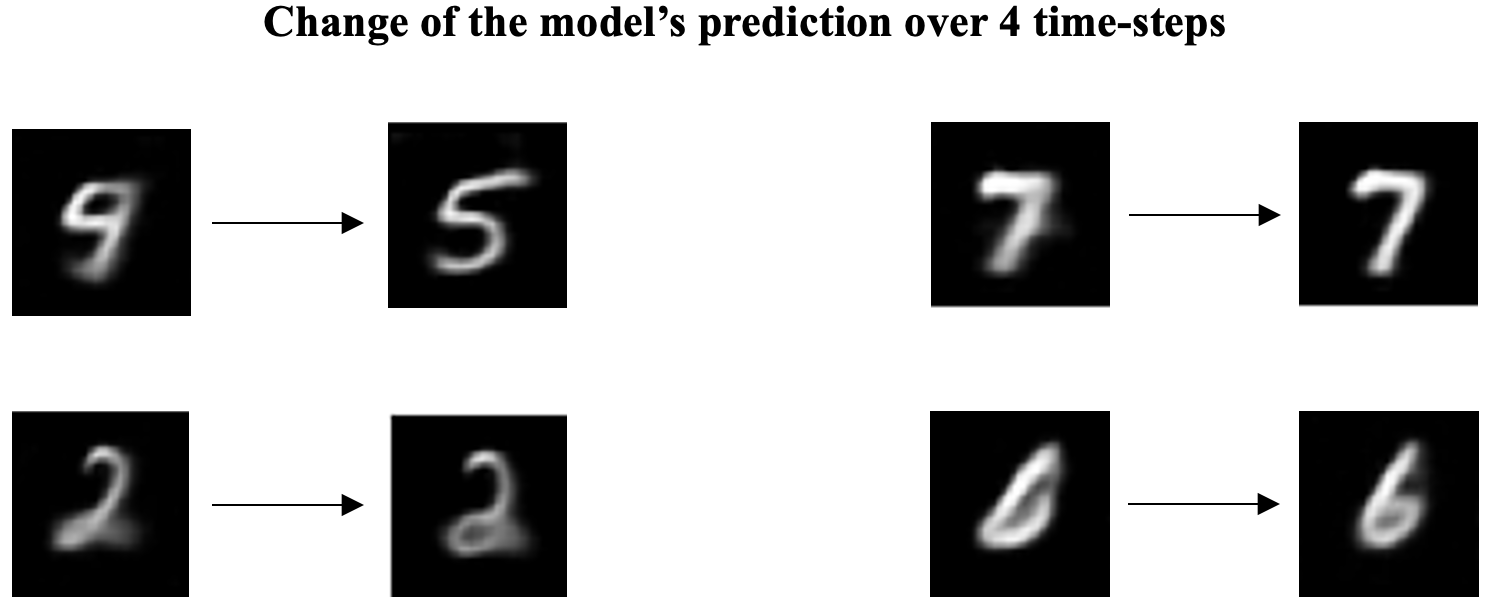
\includegraphics[width=0.79\textwidth]{hso_over_time}
    \caption[Change of the model's prediction over time]{Four random predictions of model (vi) over $4$ time-steps: The initial prediction is shown on the left and the prediction after $4$ communication cycles on the right.}
    \figlbl{hso_over_time}
\end{figure}

Of particular interest in this evaluation is not how well the samples are reconstructed but how well the latent space is shaped. Visualising the $\boldsymbol{\mu}$ values is a simple way to investigate the latent space. Therefore, the $\boldsymbol{\mu}$ vectors with a length of $n=32$ are reduced to $2$ dimensions using t-SNE \sidecite{van2008visualizing} and visualised. Since $25$ VAEs are trained in this evaluation, visualising all t-SNE plots is infeasible. Instead, \figref{hso_tSNE} only shows the plot of the baseline, the plot of the model (ii) as an example of an architecture without communication, and the plot of the model (vi) as a representative example of an architecture with communication. 

As expected, the latent space of model (i) is relatively well organised and the classes are distinguishable within the latent space. In this model, only one VAE is used, which receives the entire image as input which simplifies the organisation of the latent space. Model (ii) consists of $4$ VAEs without communication. Its latent space is less well organised: the classes are no longer clearly identifiable as clusters. However, it is interesting to note that each VAE can separate certain classes better than others because of the different patch it receives as input. Considering all $4$ VAEs, each class can be relatively well identified by at least one VAE, while no VAE can identify all classes. This indicates the benefit of a communication between the VAEs.
Applying the proposed measures (i.e. communication and predicting the whole image instead of reconstructing the input patch), the arrangement of the latent space for each VAE improves significantly: almost every VAE is able to separate the classes. This supports the usefulness of the proposed measures.

\begin{figure}[h]
    \centering
    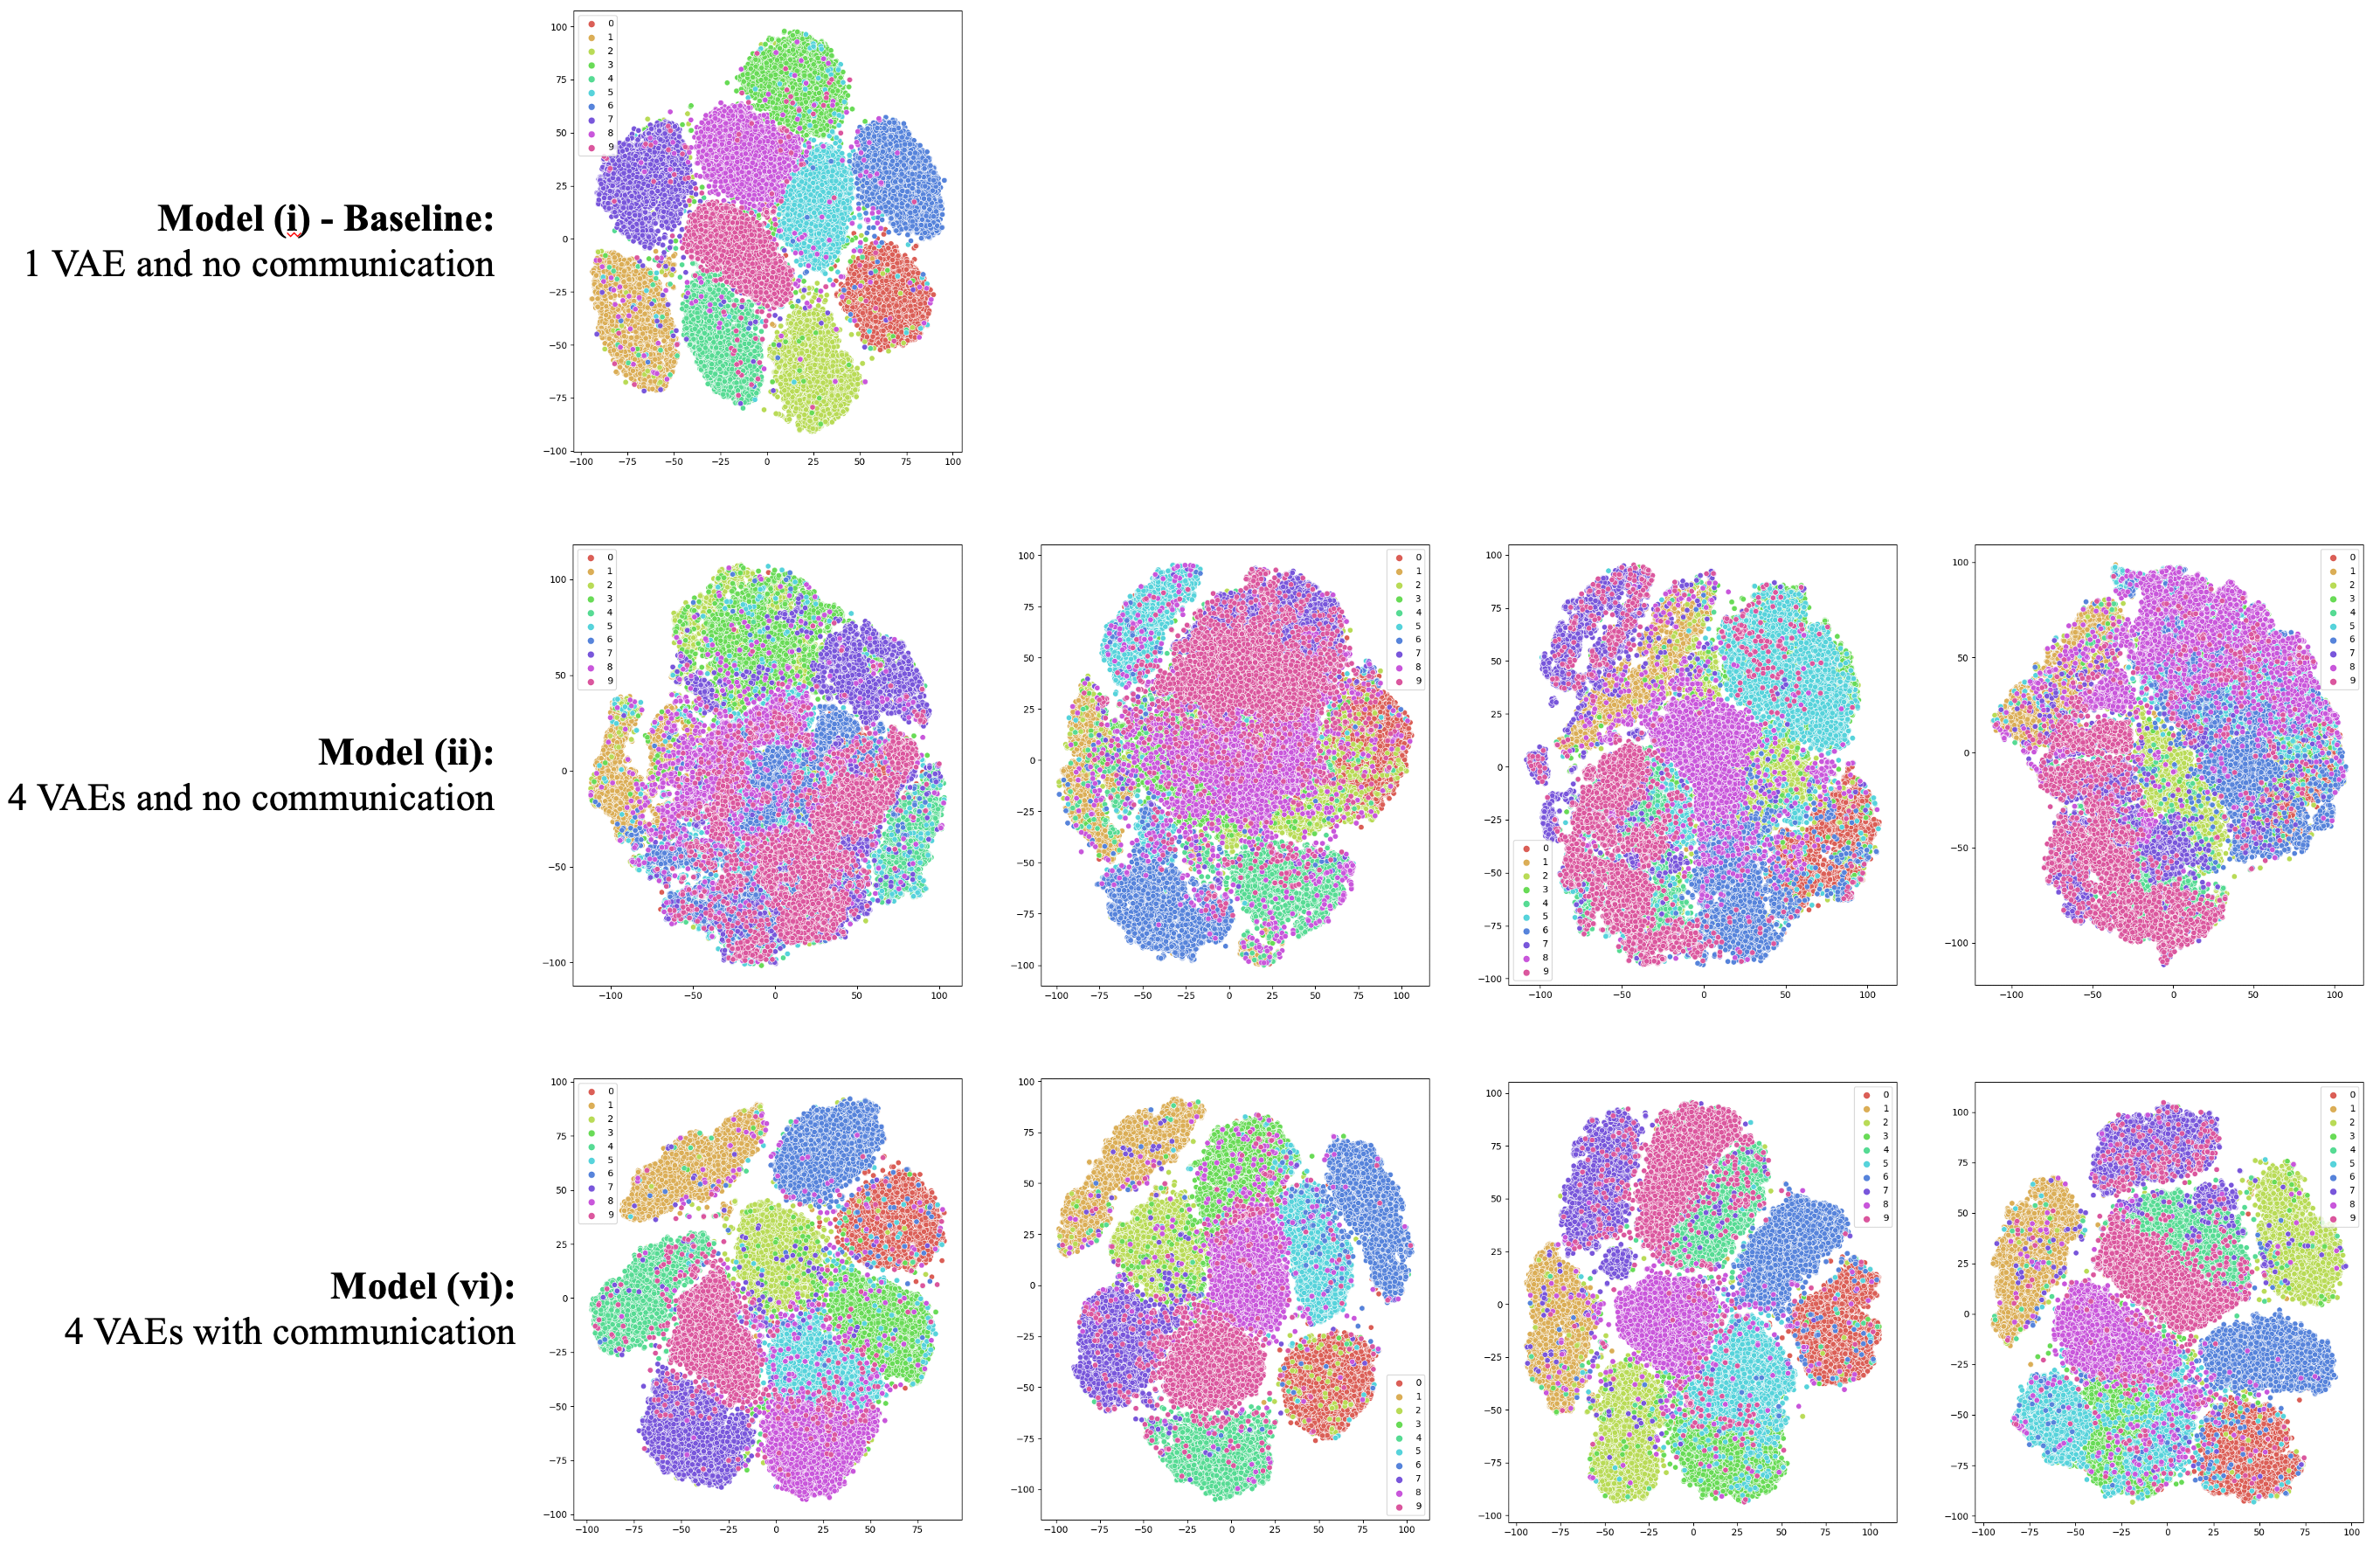
\includegraphics[width=0.99\textwidth]{hso_tSNE}
    \caption[t-SNE plot of the $\boldsymbol{\mu}$ values of different models]{t-SNE plot of the $\boldsymbol{\mu}$ values of four different models: The first row shows the baseline model ($1$ VAE), the second row the model (ii) that consists of $4$ VAEs without communication, and the third row the model (vi) that uses $4$ VAEs with communication channels. Each point in the plot corresponds to a sample, the samples are coloured according to their class.}
    \figlbl{hso_tSNE}
\end{figure}


Another way to evaluate the latent space is to measure its suitability for classification. This can be done by applying a k-means clustering and then calculating the normalised mutual information (NMI) score between the cluster centres and the labels. This metric allows the comparison between cluster assignments and labels by calculating the consistency. This means that it measures how clearly a cluster can be assigned to a label. \tabref{hso_nmi} shows the NMI scores of the models.
The NMI score is difficult to interpret as a number, and it is unclear exactly what, for example, a score of $0.6$ means for model (i). However, a relative comparison of the scores is of interest for this evaluation. The model (i) is a single VAE that receives the entire image as input, not just a patch of it. Therefore, this model is assumed to have a well-formed latent space, and the value of $0.6$ is close to an upper bound for a good latent space in this setting.

It is evident that the latent space is significantly better shaped when the whole image is predicted and not only the input patch is reconstructed. For example, models (ii) and (iii) as well as (iv) and (v) are the same models but one of the models reconstructs the input patch and the other one predicts the entire image. The models that predict the whole image are significantly better: the NMI value increases on average from $0.36$ to $0.53$ (model (ii) $\rightarrow$ model (iii)) and from $0.37$ to $0.59$ (model (iv) $\rightarrow$ model (v)) respectively.

A slight improvement through communication can also be observed. Model (iii) consists of $4$ VAEs without communication and predicts the whole picture. It achieves an NMI value of $0.53$. The models with communication are all better, reaching NMI values of $0.59$ (model (v)), $0.54$ (model (vi)) and $0.54$ (model (vii)). However, the improvement is not as clear as for the prediction of the whole image. This is probably due to the fact that the image patches are too large and more VAEs should be used. For example, model (iii) has a very high NMI score compared to the baseline, indicating that this model is able to classify and therefore the image patches contain too much image information. This makes communication less important and the results are not significantly improved by adding communication.


\begin{table}[h] 
    \tablbl{hso_nmi}
    \centering
	 \begin{tabular}{l l l l}
    	\textbf{No.} & \textbf{Avg. NMI} & \textbf{Min. NMI} & \textbf{Max. NMI}\\
        \hline
		i & $0.60$ & $0.60$ & $0.60$ \\
		ii & $0.36$  & $0.29$ & $0.39$ \\
		iii & $0.53$ & $0.49$ & $0.56$ \\
		iv & $0.37$ & $0.33$ & $0.41$\\
		v & $0.59$ & $0.58$ & $0.61$ \\
		vi & $0.54$ & $0.49$ & $0.60$ \\
		vii & $0.54$ & $0.49$ & $0.59$\\
    \end{tabular}
    \caption[NMI score of different architectures]{The NMI score between the $\boldsymbol{\mu}$ cluster centres and the ground-truth label. The clusters are calculated by using the k-means algorithm. Most models consist of several VAEs, therefore the average, minimum and maximum NMI values are reported for all VAEs per model.}
\end{table}

Finally, the proposed classification method is evaluated. For this purpose, the accuracy on the MNIST and MNIST-C data sets is determined for each model. The results are shown in \tabref{hso_accuracy}.
For each VAE of a model, the cosine similarity according to \eqref{hso_13} between a sample and a class prototype is calculated. Thus, the accuracy can not only be calculated for the entire model (i.e. all $4$ VAEs together), but also for each VAE independently. \tabref{hso_accuracy} shows the average accuracy per VAE in the column ``Avg. VAEs''. Furthermore, by calculating the average cosine-similarity a voting over all VAEs is performed and the actual model accuracy os obtained. The accuracy of this voting is shown in the column ``Overall''. The voting works exceptionally well: for example, model (ii) has $4$ VAEs with an average accuracy of $62.4\%$ on the MNIST dataset. The best VAE has an accuracy of $66.1\%$, the worst $59.7\%$. By voting, the overall accuracy increases to $81.7\%$, which is significantly better than the best VAE.

On the MNIST data set, the base model (i) is significantly outperformed by some models in terms of accuracy, but robustness (measured on MNIST-C) is not significantly improved by using multiple VAEs. As with the evaluation of the NMI score, it can be observed that models that predict the entire image perform better than models that only reconstruct a patch of the image. Furthermore, the accuracy of the models without communication is generally very high, suggesting that the image patches are too large and more VAEs should be used.



\begin{table}[h] 
    \tablbl{hso_accuracy}
    \centering
	 \begin{tabular}{l l l l l}
	 	& \textbf{Avg. VAEs} & \textbf{Overall} & \textbf{Avg. VAEs} & \textbf{Overall}\\
    	\textbf{No.} & \textbf{MNIST} & \textbf{MNIST} & \textbf{MNIST-C} & \textbf{MNIST-C}\\
        \hline
		i & - & $85.2\%$ & - & $63.4\%$ \\
		ii & $62.4\%$ & $81.7\%$ & $42.3\%$ & $60.9\%$ \\
		iii & $78.2\%$ & $89.9\%$ & $45.4\%$ & $64.9\%$ \\
		iv & $63.8\%$ & $82.6\%$ & $41.8\%$ & $60.5\%$  \\
		v & $86.1\%$ & $87.6\%$ & $62.4\%$ & $65.2\%$ \\
		vi & $88.4\%$ & $91.1\%$ & $50.4\%$ & $59.2\%$ \\
		vii & $78.5\%$ & $90.0\%$ & $46.8\%$ & $64.2\%$ \\
    \end{tabular}
    \caption[Accuracy of different architectures on MNIST and MNIST-C]{The accuracy of different models on MNIST and MNIST-C. For both data sets, the average accuracy per VAE and the overall accuracy is reported. The average per VAE is the average accuracy when each VAE makes a prediction on its own (i.e. choosing the highest cosine similarity per VAE according to \eqref{hso_13}). The overall accuracy is calculated by averaging the cosine similarity according to \eqref{hso_14}.}
\end{table}

The accuracy was calculated by comparing a sample with \emph{one} prototype per class. However, using only one prototype seems to be not enough. For example, when looking at the t-SNE plots in \figref{hso_tSNE}, the same class is divided into more than one cluster. The calculation of the NMI score also indicates that one prototype per class is insufficient: When more clusters are used for k-means clustering, the NMI scores become higher. This is also in line with the analysis of the data and the findings of vertical self-organisation (c.f. \secref{future_vso}).



TODO: Model Head is missing in this evaulation




%TODO: vereinheitliche Mathe: Was ist underline, was ist hochgestellt in Klammern ($z^{(i)}$) und was ist hochgestellt in eckigen Klammern? Bei NN: Was ist n, was ist m, ... (+ Lernraten Symbol, Loss Symbol, etc.)
%Sind alle Vektoren bold?

% TODO: target function und objective function vereinheitlichen
% TODO: net-fragment or net fragment, dataset or data set, time-step or time step

